%%%%%%%%%%%%%%%%%%%%%%%%%%%%%%%%%%%%%%%%%%%%%%%%%%%%%%%%%%%%%%%%%%%%%%%%%%%%%%%
%% Descr:       Vorlage für Berichte der DHBW-Karlsruhe
%% Author:      Prof. Dr. Jürgen Vollmer, vollmer@dhbw-karlsruhe.de
%% $Id: bericht.tex,v 1.19 2016/03/16 16:59:41 vollmer Exp $
%%  -*- coding: utf-8 -*-
%%%%%%%%%%%%%%%%%%%%%%%%%%%%%%%%%%%%%%%%%%%%%%%%%%%%%%%%%%%%%%%%%%%%%%%%%%%%%%%

\documentclass[
ngerman          % neue deutsche Rechtschreibung
,a4paper          % Papiergrösse
% ,twoside          % Zweiseitiger Druck (rechts/links)
% ,10pt             % Schriftgrösse
,11pt
% ,12pt
,pdftex
%  ,disable         % Todo-Markierungen auschalten
]{report}

% Bitte die Codierung Ihrer Dateien auswählen:
% \usepackage[latin1]{inputenc}    % Für UNIX mit ISO-LATIN-codierten Dateien
% \usepackage[applemac]{inputenc}  % Für Apple Mac
% \usepackage[ansinew]{inputenc}   % Für Microsoft Windows
\usepackage[utf8]{inputenc}        % UTF-8 codierte Dateien
% Dieses Dokument ist unter Unix erstellt, daher
% wird diese Input-Codierung benutzt.
\usepackage{setspace}
\usepackage{bericht}
\usepackage{titlesec} 
\usepackage{amsmath}
\usepackage{multirow}
\usepackage{eurosym}
\titleformat{\chapter}{\bfseries\Huge}{\thechapter.\quad}{0em}{}

%%%%%%%%%%%%%%%%%%%%%%%%%%%%%%%%%%%%%%%%%%%%%%%%%%%%%%%%%%%%%%%%%%%%%%%%%%%%%%%
%% Angaben zur Arbeit
%%%%%%%%%%%%%%%%%%%%%%%%%%%%%%%%%%%%%%%%%%%%%%%%%%%%%%%%%%%%%%%%%%%%%%%%%%%%%%%

\newcommand{\Autor}{Robin Baumann, Tom Ganz, Carlo Götz}
\newcommand{\MatrikelNummer}{}
\newcommand{\Kursbezeichnung}{TINF15B5}

\newcommand{\FirmenName}{}
\newcommand{\FirmenStadt}{}
\newcommand{\FirmenLogoDeckblatt}{
\includegraphics[width=4cm]{images/GI_InformatiCup}}

% Falls es kein Firmenlogo gibt:
%  \newcommand{\FirmenLogoDeckblatt}{}

\newcommand{\BetreuerFirma}{}
\newcommand{\BetreuerDHBW}{Prof. Dr. Johannes Freudenmann}

%%%%%%%%%%%%%%%%%%%%%%%%%%%%%%%%%%%%%%%%%%%%%%%%%%%%%%%%%%%%%%%%%%%%%%%%%%%%%%%%%%%%%

\newcommand{\Was}{Studienarbeit}
% Wird auf dem Deckblatt in der Erklärung benutzt

%%%%%%%%%%%%%%%%%%%%%%%%%%%%%%%%%%%%%%%%%%%%%%%%%%%%%%%%%%%%%%%%%%%%%%%%%%%%%%%%%%%%%

\newcommand{\Titel}{InformatiCup 2018 - IntelliTank}
\newcommand{\AbgabeDatum}{22. Mai 2018}

\newcommand{\Dauer}{3. Studienjahr}

% \newcommand{\Abschluss}{Bachelor of Engineering}
\newcommand{\Abschluss}{Bachelor of Science}

% \newcommand{\Studiengang}{Informationstechnik}
\newcommand{\Studiengang}{Angewandte Informatik}

\hypersetup{%%
	pdfauthor={\Autor},
	pdftitle={\Titel},
	pdfsubject={\Was}
}

%%%%%%%%%%%%%%%%%%%%%%%%%%%%%%%%%%%%%%%%%%%%%%%%%%%%%%%%%%%%%%%%%%%%%%%%%%%%%%%

% Wenn \includeonly{..} benutzt wird, werden nur diese Kaptitel ausgegeben.

%%%%%%%%%%%%%%%%%%%%%%%%%%%%%%%%%%%%%%%%%%%%%%%%%%%%%%%%%%%%%%%%%%%%%%%%%%%%%%%
% Benutzt man das "biblatex"-Paket, dann muß das hier stehen:
% siehe auch die mit BIBLATEX markierten Zeilen in bericht.sty
\addbibresource{bericht.bib}

\usepackage{fancyhdr}
\pagestyle{fancy}
\fancyhf{}
\fancyhead[R]{\Titel}
\renewcommand{\headrulewidth}{0.4pt} %obere Trennlinie
\renewcommand{\footrulewidth}{0.4pt} %untere Trennlinie
\fancyfoot[R]{\thepage} %Seitennummer
\fancyfoot[L]{\Autor \vspace{1ex} | TINF15B5}
\fancypagestyle{plain}{}% damit auch "plain" Seiten fancy werden

% argmin command for math env
\DeclareMathOperator*{\argmin}{arg\,min}

\begin{document}
\pagenumbering{Roman}

%%%%%%%%%%%%%%%%%%%%%%%%%%%%%%%%%%%%%%%%%%%%%%%%%%%%%%%%%%%%%%%%%%%%%%%%%%%%%%%

\begin{titlepage}
	\begin{center}
		\vspace*{-2cm}
		\FirmenLogoDeckblatt\hfill
\includegraphics[width=4cm]{images/dhbw-logo}\\[2cm]
		{\Huge \Titel}\\[2cm]
		{\Huge\scshape \Was}\\[2cm]
		{\large für die Prüfung zum}\\[0.5cm]
		{\Large \Abschluss}\\[0.5cm]
		{\large des Studienganges \Studiengang}\\[0.5cm]
		{\large an der}\\[0.5cm]
		{\large Dualen Hochschule Baden-Württemberg Karlsruhe}\\[0.5cm]
		{\large von}\\[0.5cm]
		{\large\bfseries \Autor}\\[1cm]
		{\large Abgabedatum \AbgabeDatum}
		\vfill
	\end{center}
	\begin{tabular}{l@{\hspace{2cm}}l}
		Zeitraum	         & \Dauer 			\\
		Kurs			         & \Kursbezeichnung		\\
		%Betreuer der Ausbildungsfirma	 & \BetreuerFirma		\\
		Gutachter der Studienakademie	 & \BetreuerDHBW		\\
	\end{tabular}
\end{titlepage}

%%%%%%%%%%%%%%%%%%%%%%%%%%%%%%%%%%%%%%%%%%%%%%%%%%%%%%%%%%%%%%%%%%%%%%%%%%%%%%%

% Nur für Bachelorarbeiten einfügen:
%%%%%%%%%%%%%%%%%%%%%%%%%%%%%%%%%%%%%%%%%%%%%%%%%%%%%%%%%%%%%%%%%%%%%%%%%%%%%%%
%% Descr:       Vorlage für Berichte der DHBW-Karlsruhe, Erklärung
%% Author:      Prof. Dr. Jürgen Vollmer, vollmer@dhbw-karlsruhe.de
%% $Id: erklaerung.tex,v 1.6 2016/03/16 12:51:09 vollmer Exp $
%% -*- coding: utf-8 -*-
%%%%%%%%%%%%%%%%%%%%%%%%%%%%%%%%%%%%%%%%%%%%%%%%%%%%%%%%%%%%%%%%%%%%%%%%%%%%%%%

% In Bachelorarbeiten muss eine schriftliche Erklärung abgegeben werden.
% Hierin bestätigen die Studierenden, dass die Bachelorarbeit, etc.
% selbständig verfasst und sämtliche Quellen und Hilfsmittel angegeben sind. Diese Erklärung
% bildet das zweite Blatt der Arbeit. Der Text dieser Erklärung muss auf einer separaten Seite
% wie unten angegeben lauten.

\newpage
\thispagestyle{empty}
\begin{framed}
\begin{center}
\Large\bfseries Erklärung
\end{center}
\medskip
\noindent
Wir versichern hiermit, dass wir unsere \Was\ mit
dem Thema: \enquote{\Titel} selbstständig verfasst und keine anderen als die angegebenen Quellen und
Hilfsmittel benutzt haben. Wir versichern zudem, dass die eingereichte elektronische Fassung mit der
gedruckten Fassung übereinstimmt.

\vspace{3cm}
\noindent
\underline{\hspace{4cm}}\hfill\underline{\hspace{10.5cm}}\\
Ort~~~~~Datum\hfill Unterschriften\hspace{4cm}
\end{framed}

\vfill


%%%%%%%%%%%%%%%%%%%%%%%%%%%%%%%%%%%%%%%%%%%%%%%%%%%%%%%%%%%%%%%%%%%%%%%%%%%%%%%
\endinput
%%%%%%%%%%%%%%%%%%%%%%%%%%%%%%%%%%%%%%%%%%%%%%%%%%%%%%%%%%%%%%%%%%%%%%%%%%%%%%%


\newpage

\begingroup
\parskip=-1pt
\tableofcontents
\endgroup

\begingroup
\renewcommand\clearpage{\relax}
\listoffigures
\listoftables
\endgroup              % Liste der Tabellen
% \lstlistoflistings         % Liste der Listings
%\listofequations           % Liste der Formeln

% Jetzt kommt der "eigentliche" Text
%%%%%%%%%%%%%%%%%%%%%%%%%%%%%%%%%%%%%%%%%%%%%%%%%%%%%%%%%%%%%%%%%%%%%%%%%%%%%%
%% Descr:       Vorlage für Berichte der DHBW-Karlsruhe, Datei mit Abkürzungen
%% Author:      Prof. Dr. Jürgen Vollmer, vollmer@dhbw-karlsruhe.de
%% $Id: abk.tex,v 1.3 2016/03/16 12:21:40 vollmer draft $
%% -*- coding: utf-8 -*-
%%%%%%%%%%%%%%%%%%%%%%%%%%%%%%%%%%%%%%%%%%%%%%%%%%%%%%%%%%%%%%%%%%%%%%%%%%%%%%%

\chapter*{Abkürzungsverzeichnis}                   % chapter*{..} -->   keine Nummer, kein "Kapitel"
						         % Nicht ins Inhaltsverzeichnis
% \addcontentsline{toc}{chapter}{Akürzungsverzeichnis}   % Damit das doch ins Inhaltsverzeichnis kommt

% Hier werden die Abkürzungen definiert
%\begin{acronym}[DHBW]
  % \acro{Name}{Darstellung der Abkürzung}{Langform der Abkürzung}
%\end{acronym}

\begin{acronym}
	\acro{API}{Application Programming Interface}
	\acro{ARMA}{Autoregressive-Moving Average}
	\acro{ARIMA}{Autoregressive Integrated Moving Average}
	\acro{CLI}{Command Line Interface}
	\acro{CORS}{Cross-Origin Resource Sharing}
	\acro{CSV}{Comma Separated Values}
	\acro{DI}{Dependency Injection}
	\acro{HTTP}{Hypertext Transfer Protocol}
	\acro{IOC}{Inversion Of Control}
	\acro{JSF}{Java Server Faces}
	\acro{JSON}{Javascript Object Notation}
	\acro{MAE}{Mean Absolute Error}
	\acro{OSM}{Open Street Map}
	\acro{RDBMS}{Relational Database Management System}
	\acro{RMSE}{Root Mean Squared Error}
	\acro{SPA}{Single Page Application}
\end{acronym}              % Abkürzungsverzeichnis




\pagenumbering{arabic}
\setcounter{page}{1}

%-------------------------------------------------------------------------------
% BODY
%-------------------------------------------------------------------------------
\pagenumbering{arabic}

\chapter{Einleitung}

\section{InformatiCup}

Die hier beschriebene Arbeit behandelt die Lösung der Aufgabe IntelliTank. Diese ist Bestandteil des 13. InformatiCup-Wettbewerbs, welcher von der Gesellschaft für Informatik e.V. jährlich organisiert wird.
Anlässlich des InformatiCups treten Teams aus verschiedenen Universitäten und Hochschulen gegeneinander an, um Ihre Lösungen vorzustellen. Die besten vier werden durch eine Jury gekürt und erhalten einen Preis, sowie eine Einladung zu einer Fachtagung der Gesellschaft für Informatik, auf welcher sie ihre Lösung einem Publikum präsentieren dürfen.

\section{Aufgabenstellung}

Die diesjährige Problemstellung trägt den Namen IntelliTank. Aufgabe ist es, ein Modell zur Vorhersage zukünftiger Benzinpreis(Superkraftstoff E5)-Entwicklungen an allen Tankstellen Deutschlands zu entwickeln. Die Vorhersagen sollen dabei bis zu einem Monat voraus mit einer gewissen Signifikanz berechnet werden. Als Grundlage dieser Arbeit wird von Tankerkönig.de eine Datenbasis zur Verfügung gestellt. Diese beinhaltet die unbereinigten historischen Benzinpreise von rund 15.000 Tankstellen in Deutschland seit 2013. Mithilfe dieser Grundlage ist es möglich eine Korrelationsanalyse durchzuführen. Zusätzlich können weitere Datenquellen mit in das Modell einbezogen werden, um die allgemeine Vorhersagegüte des statistischen Modells zu verbessern.\\

%TODO: Bitte nochmal umformulieren. Sonst einfach Copy Paste aus der Aufgabenstellung der GI.
Abhängig davon soll eine Anwendung entworfen werden, welche auf Basis des Vorhersagemodells zu einer gegebenen Route eine optimale Tankstrategie liefert.
Zur Einfachheit wird eine Route definiert, durch verschiedene Stopps an Tankstellen und dem jeweiligen Zeitpunkt an den man ihn erreicht. Die Anwendung soll also zu diesen Zeitpunkten der jeweiligen Tankstelle einen vorhergesagten Preis festlegen und als Ergebnis zu jeder Tankstelle eine optimale Menge Benzin ermitteln.

\section{Motivation}
Das Auto ist in Deutschland das Fortbewegungsmittel Nummer 1. Einer Umfrage des Umweltbundesamtes (UBA) zufolge sind 37 Prozent der Menschen in Deutschland (ab 14 Jahre) täglich mit dem Kfz unterwegs \cite{fortbewegung}. Außerdem gibt ein Privathaushalt in Deutschland jeden Monat rund 100 Euro für Autokraftstoff aus. Auch wenn die Elektromobilität stark auf dem Vormarsch ist, besitzen die meisten Deutschen noch ein Fahrzeug mit einem Verbrennungsmotor. Durch eine intelligente, vorausschauende Tankstrategie lässt sich bares Geld sparen. 


\chapter{Theoretische Grundlagen}

In diesem Kapitel werden die theoretischen Grundlagen zur in dieser Arbeit vorgestellten Lösung zum 13. InformatiCup der Gesellschaft für Informatik e.V. vorgestellt. Zunächst wird das Fixed-Path-Gas-Station Problem erklärt, welches die Basis des zu entwerfenden Routing-Algorithmus darstellt. Anschließend werden die Grundlagen der Zeitreihenanalyse und Regressionsanalyse vorgestellt.

\section{Fixed-Path-Gas-Station Problem}

Die hier verwendete Tankstrategie wurde implementiert nach dem Algorithmus aus der Publikation 'To Fill or Not To Fill'\cite{fixedgas}.
Gegeben sei eine Route, welche definiert ist durch eine Menge von Tankstellen und eine maximale Tankkapazität des Fahrzeuges.
Jede Tankstelle ist abzufahren, wobei die erste Tankstelle dem Startpunkt der Route entspricht. In Abbildung \ref{fig:fixedgas} ist eine Visualisierung des Problems zu erkennen. In unserer Problemstellung ist der Pfad jedoch festgelegt und kann nicht geändert werden, somit ist das Problem des 'Shortest-Path' zu vernachlässigen. 
Dadurch ergibt sich folgender Algorithmus:
\begin{enumerate}
\item Sei $b$ die aktuelle Position gegeben durch eine Tankstelle
\item Sei $l$ eine Liste von Tankstellen die durch die maximale Tankkapazität von $b$ aus erreichbar sind
\item Sortiere die Liste nach den Benzinpreisen und der Nähe zum Ziel aufsteigend
\item Tanke genau so viel, dass die günstigste (erste) Tankstelle $c$ aus $l$ erreicht wird
\item Falls $c$ nicht die End-Tankstelle ist, wiederhole Punkt $1$
\end{enumerate}

\begin{figure}
	\centering
	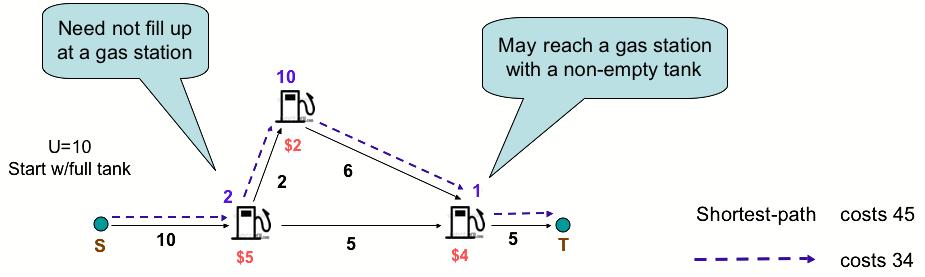
\includegraphics[width=0.8\linewidth]{images/fixedgas}
	\caption[Beispiel Ablauf]{\textit{Visualisierung des Problems \cite{fixedgasimage}}} 
	\label{fig:fixedgas}
\end{figure}



Ebenfalls benutzen wir eine naive Tankstrategie (immer volltanken) um sie mit unserer zu vergleichen. Der Algorithmus wird beschrieben durch:

\begin{enumerate}
\item Sei $l_{i=0}$ die aktuelle Position gegeben durch eine Tankstelle
\item Tanke voll (Kapazität-Füllstand)
\item Erreiche die nächste Tankstelle $l_{i+1}$
\item Tanke die während der Distanz von $l_{i}$ nach $l_{i+1}$ verbrauchten Liter wieder auf
\item Falls $l_{i+1}$ nicht die End-Tankstelle ist, wiederhole Punkt $3$
\end{enumerate}

Die Distanz zwischen zwei Tankstellen wird mittels der Haversine-Formel zwischen zwei Geo-Punkten berechnet \cite{haversine}.\\
Die Berechnung der Haversine-Formel ist gegeben durch
$$ \Delta longitude = longitude_b - longitude_a $$
$$ \Delta latitude = latitude_b - latitude_a $$
$$ a = (\frac{\sin \Delta latitude}{2})^2 + \cos latitude_a * \cos latitude_b * (\frac{\sin \Delta longitude}{2}^2)$$
$$ c = 2 * \arcsin \min(1,\sqrt{a})$$
$$ d = R * c $$
Wobei $R$ dem Erdradius entspricht.\\
Die Haversine-Formel ermöglicht die Berechung der Distanz zweier Geokoordinate auf einer Kugel-Oberfläche (sogenannte Orhodrome).

\subsection{Implementierung}

Unsere Lösung für das Fixed-Path-Gas-Station Problem lässt sich in einem Algorithmus implementieren der eine Zeitkomplexität von $O(n*log (n))$ benötigt\cite{fixedgas}. Hierzu wird eine Priority-Queue mit allen Stationen befüllt, welche man mit einem vollen Tank von einer Initial-Tankstelle $l_0$ aus erreichen kann.
Diese Priority-Queue wird ähnlich einem 'Moving Window' von Station zu Station in Richtung Ziel-Tankstelle 'geschoben'.
Die Priority-Queue speichert jede Tankstelle innerhalb der Queue abhängig ihres Preises.
Um die nächste Tankstelle von unserer Start-Tankstelle $l_0$ aus zu ermitteln, wird die nächste Tankstelle $l_1$ mit der höchsten Priorität aus der Queue entnommen.
Jedes mal wenn wir das Fenster um eine Tankstelle verschieben wird die Start-Tankstelle entfernt und alle Tankstellen die von $l_{0_{neu}}$ aus erreichbar sind zur Queue hinzugefügt. Da das Entfernen und Hinzufügen in $O(log (n))$ verrichtet werden kann\cite{queue}, entspricht der Aufwand das Problem zu lösen $O(n*log (n))$. Um zu beweisen, dass die Lösung optimal ist, muss nach dem Bellman'schen Optimalitätsprinzip\cite{bellman} nur bewiesen werden, dass jedes Subproblem (Zwischenroute) $l_i$ zu $l_{i+1}$ optimal ist. Diese ist es, falls der Tank $l_i$ genau dem entspricht, was zum Erreichen von der nächst günstigsten Tankstelle $l_{i+1}$ notwendig ist, also wenn am ende der Tank leer ist. 

\section{Zeitreihenanalyse}
Bei einer Zeitreihe handelt es sich um eine zeitlich geordnete Sequenz von Messungen eines Systems \cite[145]{thinkstats}. Das in dieser Arbeit behandelte Problem kann als eine Zeitreihenanalyse betrachtet werden. Viele Algorithmen zur Analyse von Zeitreihen funktionieren stabiler, wenn die zu untersuchende Zeitreihe mit einer gleichmäßigen Frequenz vorliegt \cite[146]{thinkstats}. Dies ist nicht immer gegeben. In dem verwendeten Datensatz sind die Benzinpreise zu den jeweiligen Änderungszeitpunkten in der Datenbank gespeichert. Aus diesem Grund wechseln die Abstände zwischen zwei aufeinanderfolgenden Messungen von wenigen Minuten bis zu mehreren Stunden. Manche Tankstellen weisen sogar Lücken von mehreren Tagen auf. Aus diesem Grund ist eine Vorverarbeitung des Datensatzes notwendig, um die Messungen auf eine einheitliche Frequenz zu bringen. Genaueres hierzu wird in Abschnitt \ref{feng} erläutert. Auf den vorbereiteten Daten lassen sich nun unterschiedliche Methoden zur Analyse der Zeitreihe anwenden, welche nachfolgend beschrieben werden.

\subsection{Gleitende Durchschnitte}
Die meisten Zeitreihen setzen sich aus den folgenden drei Komponenten zusammen \cite[151]{thinkstats}:

\begin{enumerate}
	\item \textit{Trend}: Systematische zu- oder Abnahme.
	\item \textit{Saisonalität}: Periodische Schwankungen.
	\item \textit{Fluktuation}: Zufällige Abweichungen vom Langzeittrend.
\end{enumerate}
Zur Analyse der zugrundeliegenden Zeitreihe werden diese einzelnen Komponenten sukzessive, nicht simultan eliminiert \cite[397]{lippe}. Bei der Methode der gleitenden Durchschnitte wird dabei der Trend der zugrundeliegenden Zeitreihe berechnet. Gleitende Durchschnitte werden dabei als eine Folge arithmetischer Mittel von jeweils $p$ aufeinanderfolgenden Werten der Zeitreihe gebildet werden \cite[403]{lippe}. Durch den p-gliedrigen gleitenden Durchschnitt entsteht eine geglättete Zeitreihe, die mit größerem p immer glatter wird. 

\subsection{Autokorrelation} \label{autokorr}
Autokorrelation beschreibt die Korrelation einer Funktion mit sich selber zu einem früheren Zeitpunkt \cite[155]{thinkstats}. Um die Saisonalität herauszufinden wird die Funktion um ein sogenanntes \textit{lag}-Intervall verschoben und auf Korrelation mit der originalen Funktion geprüft. Dies wird mit unterschiedlichen Intervallen wiederholt, um entsprechend auf tägliche, wöchentliche oder monatliche Trends schließen zu können. Für jede dieser Verschiebungen wird dann der Korrelationskoeffizient im Wertebereich [0,1] berechnet. Anhand der berechneten Werte kann eine statistische Signifikanz der eventuell enthaltenen Saisonalitäten bestimmt werden.

\subsection{\acf{ARMA}-Modelle}
Ein \ac{ARMA}(p, q)- Modell setzt sich aus einem Autoregressiven AR(p) - und einem Moving Average MA(q)-Modell zusammen \cite[18]{timeseries}. Die Autoregressive Komponente berechnet zukünftige Werte aus der Linearkombination von p historischen Messwerten, einem zufälligen Fehler $\epsilon$ und einer Konstante $c$. Mathematisch wird das wie folgt formuliert:

\begin{equation}
	y_t = c + \sum_{i=1}^{p}\phi_i y_{t-i} + \epsilon_t
\end{equation}

Die Werte $\phi_i$\ $(i = 1, 2, ..., p)$ sind Modellparameter. Das MA(q)-Modell benutzt vergangene Fehler des Modells als erklärende Variable \cite[19]{timeseries} und ist wie folgt definiert:

\begin{equation}
	y_t = \mu + \sum_{i=1}^{q} \Theta_i \epsilon_{t-i} + \epsilon_t
\end{equation}

In dieser Definition beschreibt $\mu$ den Mittelwert über $q$ gleitende Durchschnitte und $\Theta_i$\ $(i=1, 2, ..., q)$ sind Modellparameter. Die Fluktuationen werden als standardnormalverteilt angenommen. Konzeptuell entspricht das Moving-Average Modell also einer linearen Regression des aktuell betrachteten Messwertes gegen die Fluktuationen eines oder mehrerer früherer Messwerte(s) \cite[19]{timeseries}. Die Kombination der beiden Einzelmodelle liefert dann das gewünschte \ac{ARMA}(p,q)-Modell, welches eine Vorhersage nach folgender mathematischen Vorschrift berechnet:

\begin{equation}
	y_t = c + \epsilon_t + \sum_{i=1}^{p}\phi_i y_{t-i} + \sum_{i=1}^{q} \Theta_i \epsilon_{t-i}
\end{equation} 

\subsection{Stationarität}
Üblicherweise werden \ac{ARMA}-Modelle mit dem Lag-Operator definiert \cite[19]{timeseries}, welcher mathematisch als $Ly_t = y_{t-1}$ definiert ist. Somit lassen sich \ac{ARMA}-Modelle mittels Lag-Polynomen wie folgt definieren:

\begin{equation*}
	AR(p)-Modell: \epsilon_t = \phi(L)y_t 
\end{equation*}
\begin{equation*}	
	MA(q)-Modell: y_t = \Theta(L)\epsilon_t \
\end{equation*}
\begin{equation}
	ARMA(p, q)-Modell: \phi(L)y_t = \Theta(L)\epsilon_t
\end{equation}

In diesem Fall gilt:
\begin{equation*}
	\phi(L) = 1-\sum_{i=1}^{p}\phi_i L_i \text{\hspace{2em} und \hspace{2em}}
	\Theta(L) = 1 + \sum_{j=1}^{q} \Theta_j L_j
\end{equation*}

Ein solches Modell wird als stationär bezeichnet, genau dann wenn die Modellparameter Zeitunabhängig sind \cite[160]{thinkstats}. Ein \ac{ARMA}(p,q)-Modell ist stationär, wenn für alle Wurzeln aus der charakteristischen Gleichung $\phi(L) = 0$ außerhalb des Einheitskreises liegen \cite[20]{timeseries}. \ac{ARMA}-Modelle arbeiten nur auf stationären Zeitreihen zuverlässig. \\
\par 

Von Natur aus besitzen viele Zeitreihen ein nicht-stationäres Verhalten. Dies ist inhärent durch den Trend und die Saisonalität einer Zeitreihe gegeben. Aus diesem Grund können für den in dieser Arbeit verwendeten Datensatz keine einfachen \ac{ARMA}-Modelle verwendet werden. Es gibt jedoch Erweiterungen dieser \ac{ARMA}-Modelle, welche mit nicht stationären Zeitreihen umgehen können. Eine dieser Erweiterungen stellen die \ac{ARIMA}-Modelle dar, welche nachfolgend kurz beschrieben werden.

\subsection{\acf{ARIMA}-Modelle}
In \ac{ARIMA}-Modellen wird die Stationarität der Zeitreihe durch finite-Differenzierung erreicht. Mathematisch ist ein \ac{ARIMA}(p, d, q)-Modell wie folgt mit Hilfe der oben definierten Lag-Polynome definiert:

\begin{equation*}
	\phi(L)(1-L)^d y_t = \Theta(L)\epsilon_t
\end{equation*}
Das heißt ausformuliert:
\begin{equation}
	\left(1-\sum_{i=1}^{p}\phi_i L_i \right) (1-L)^d y_t = \left(1 + \sum_{j=1}^{q} \Theta_j L_j \right) \epsilon_t
\end{equation}

\begin{itemize}
	\item $p$, $d$ und $q$ sind dabei Integer $\geq$ 0 und bezeichnen die Ordnung der Autoregressiven- , Integrierten- und gleitenden Durchschnitts-Komponente des Modells.
	\item $d$ beschreibt das Differenziationslevel. Im Umkehrschluss erhält man durch $d$-fache Integration die Werte der ursprünglichen Zeitreihe zurück.
\end{itemize}

Durch ein geeignetes \ac{ARIMA}-Modell können auf Basis der vorhandenen Benzinpreise bereits Vorhersagen getroffen werden. Jedoch besteht der größte Nachteil dieser Modell-Klasse darin, dass Vorhersagen allein aus den historischen Daten generiert werden. Für die Lösung der Benzinpreisvorhersage sollen jedoch zusätzliche Parameter in das Vorhersagemodell eingebunden werden, um die allgemeine Vorhersagegüte zu verbessern. Aus diesem Grund wurden noch andere Modelle untersucht, mit deren Hilfe Feature-Vektoren mit zusätzlichen Parametern für die Benzinpreisvorhersage verwendet werden können. Diese Modelle nutzen Regressionsanalyse zur Vorhersage, welche nachfolgend beschrieben wird.


\section{Regressionsanalyse}
%TODO: Regression allgemein und explizit für Zeitreihenanalyse.
Das Ziel der Regressionsanalyse ist die Beschreibung der Beziehung von einem Variablensatz, genannt \textit{abhängige Variablen}, zu den sogenannten \textit{erklärenden Variablen} \cite[129]{thinkstats}. Die Regression liefert also für einen mehrdimensionalen Eingabevektor einen konkreten numerischen Wert. Der Algorithmus soll also eine Funktion $f: \mathbb{R}^n \rightarrow\ \mathbb{R}$ entwickeln. Für den Fall, dass jeweils genau eine abhängige und erklärende Variable für die Regression verwendet wird, spricht man von einer \textit{einfachen Regresssion}, bei mehr als einer erklärenden Variable wird von \textit{Multipler Regression} gesprochen \cite[129]{thinkstats}. Entsprechend dem Grad der Regressionsfunktion wird in unterschiedliche Methoden unterschieden, welche nachfolgend erläutert werden.

\subsection{Lineare Regression}
Lineare Modelle sind die einfachsten parametrischen Methoden und sollten für jede Problemstellung zunächst in Betracht gezogen werden, da sie oft auch intrinsisch nicht-lineare Probleme einfach lösen können \cite[72]{mlalgos}. Die zentrale Annahme eines linearen Modells ist dabei, dass alle Werte im Datensatz und alle anderen unbekannten Punkte auf einer Hyperebene liegen und der maximale Fehler proportional zur Trainingsqualität und Adaptivität ist \cite[73]{mlalgos}. Bei einem linearen Zusammenhang der untersuchten Variablen wird die Regressionsgerade über zwei Parameter, die sogenannten Korrelationskoeffizienten bestimmt:
\begin{equation}
	\bar{y} = \alpha + \beta x
\end{equation}

Der Parameter $\alpha$ denotiert dabei den Achsenabschnitt und $\beta$ die Steigung der Regressionsgeraden. \\
\par


\begin{figure}
	\centering
	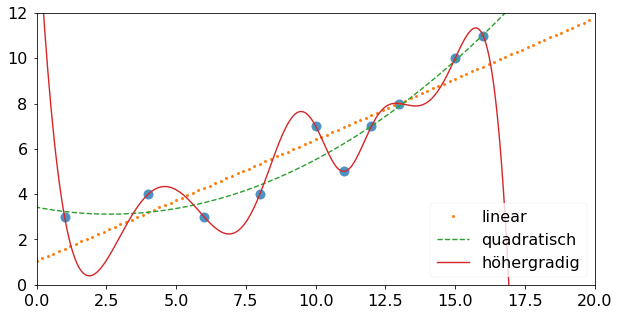
\includegraphics[width=0.7\linewidth]{images/overfit}
	\caption[Anpassungsgrad der Regressionsfunktion.]{\textit{Die hellblauen Datenpunkte werden durch die drei Regressionsfunktionen approximiert. Hier ist zu beachten, dass die lineare Funktion (Orange gepunktet) die Daten nicht gut approximiert. Die quadratische Funktion (Grün gestrichelt) approximiert den Zusammenhang gut, die höhergradige Funktion passt sich den Datenpunkten \glqq zu gut\grqq an. Man spricht hier von Overfitting. }}
	\label{fig:overfit}
\end{figure}


Gesucht ist eine möglichst gute Approximation der vorhandenen Datenpunkte durch die Regressionsfunktion. In \autoref{fig:overfit} sind drei mögliche Regressionsfunktionen zu einem Beispieldatensatz abgebildet. Es ist zu beachten, dass die lineare Funktion hier keine gute Approximation des Zusammenhangs darstellt. Die beste Approximation wird durch die höhergradige Funktion erzielt. Dies ist jedoch nicht immer das Ziel, da mit diesem Modell sehr schlecht zukünftige Werte vorhergesagt werden können. Anschaulich wird dies, wenn man sich das rechte Ende des Funktionsgraphen anschaut. Nach dem Verlauf der roten Kurve müssten alle weiteren Werte der Messreihe plötzlich stark abfallen, obwohl eigentlich ein weiterer Anstieg zu erwarten wäre. Die beste Approximation im Kontext einer Regressionsanalyse liefert daher die quadratische Funktion.

\subsection{Regression für Zeitreihenanalyse}
Wie in \cite[72]{mlalgos} erwähnt wird, stellen lineare Modelle oft einen guten Startpunkt für die Analyse vieler Probleme dar. So kann theoretisch auch eine Zeitreihenanalyse mit Hilfe eines Regressionsmodells durchgeführt werden. Jedoch ist hierbei Vorsicht geboten, denn es sprechen einige Gründe gegen die Verwendung eines Regressionsmodells bei Zeitreihenanalysen. Die folgenden drei Punkte sind \cite[150]{thinkstats} entnommen:

\begin{enumerate}
	\item Es ist in keinster Weise garantiert, dass der Langzeittrend bei einem realen Vorgang, welcher durch die Zeitreihe dokumentiert wird, einem linearen - oder höhergradigen - Modell folgt. Bezogen auf diese Arbeit bedeutet dies, dass die Benzinpreisentwicklung stark von anderen Faktoren als der Zeit abhängt. Das gebildete Modell kann somit zu einem späteren Zeitpunkt seine Gültigkeit verlieren.
	\item Die Lineare Regression gewichtet alle historischen Daten gleich stark. Die Gewichtung sollte jedoch stärker von den jüngsten Messwerten abhängen, da diese die aktuelle Entwicklung der Messreihe genauer beschreiben.
	\item Eine der Annahmen Linearer Regression ist, dass die Messfehler unkorrelierte Störungen sind. In Zeitreihenanalyse ist diese Annahme oft falsch, da aufeinanderfolgende Werte oft korrelieren. Dies wurde bereits in \autoref{autokorr} erläutert.
\end{enumerate}

Die Stärke der Regressionsanalyse gegenüber den vorgestellten \ac{ARMA}-Modellen liegt hingegen darin, dass zusätzliche Merkmale in den Merkmalsvektor zur Vorhersage künftiger Ereignisse hinzugezogen werden können. Dies kann die allgemeine Vorhersagegüte des Modells deutlich verbessern.


\chapter{Implementierungsdetails}
Zur Lösung der Aufgabenstellung wurde eine Software entwickelt, deren Aufbau im Folgenden beschrieben wird. Das Design und die Implementierung der Anwendung kann in die Teile Backend, Frontend, Fixed-Path-Gas-Station-Problem und Preisvorhersage unterteilt werden. Die einzelnen Teile werden in den nächsten Abschnitten jeweils erläutert.

\section{Backend}
Das Backend hat die Aufgabe, die benötigten Daten für das Frontend bereitzustellen. Zur Kommunikation zwischen Front- und Backend wird  \ac{HTTP} in Verbindung mit dem Datenformat \ac{JSON} verwendet. Das Backend ist dabei nicht für die Generierung einzelner Teile des Frontends zuständig, wie es bei Technologien wie \ac{JSF} der Fall ist.

Diese Entkoppelung ermöglicht die Implementierung weiterer spezialisierter Frontends. So wäre zum Beispiel die Entwicklung eines Frontends für Mobilgeräte ohne große Anpassungen des Backends möglich.

Für die Umsetzung des Backends wurde die Programmiersprache Java gewählt. Java bietet viele Open Source Bibliotheken, die die Entwicklung der Problemlösung unterstützen und beschleunigen können. Neben der großen Auswahl an Bibliotheken, bietet Java sowohl ausreichende Performance als auch viele Werkzeuge, die den Entwicklungsprozess vereinfachen. Durch die Plattformunabhängigkeit ist es auch möglich, dass die Entwicklung auf jedem der im Team eingesetzten Betriebssysteme reibungslos und ohne spezielle Anpassungen möglich ist.

Im nächsten Abschnitt wird auf die Architektur des Backends eingegangen.

\subsection{Architektur}

\begin{figure}
\centering
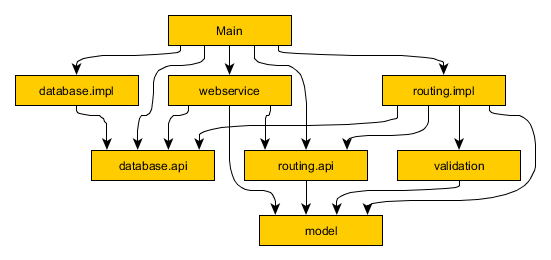
\includegraphics[width=1\linewidth]{architecture.png}
\caption{Abhängigkeiten der einzelnen Packages des Backends}
\label{fig:arch}
\end{figure}

Abbildung \ref{fig:arch} zeigt die Architektur des Backends. Es werden die einzelnen Packages und ihre Abhängigkeiten untereinander aufgeführt. \texttt{Main} ist die einzige Klasse, die nicht in einem weiteren Sub-Package enthalten ist und wird deshalb separat aufgeführt.

Zur Aufgabe von \texttt{Main} gehört es, die Applikation zu starten und die Implementierungen der einzelnen Interfaces zu instanziieren. Durch Verwendung des \ac{IOC}-Prinzips wird sichergestellt, dass die einzelnen Sub-Packages jeweils nur vom Interface abhängen und nicht von einer konkreten Implementierung des Interfaces. Die Abhängigkeiten einer Klasse werden zur Laufzeit per Constructor-Injection zur Verfügung gestellt. Auf die Verwendung eines \ac{DI}-Containers wurde verzichtet, da er bei dieser Programmgröße und -komplexität keine Vorteile bringt.

Ein Nebeneffekt dieser Aufteilung ist die Möglichkeit, Unit Tests für die einzelnen Klassen zu schreiben ohne zum Beispiel eine aktive Datenbankverbindung zu benötigen. Über Mocking Bibliotheken kann in Tests statt einer konkreten Implementierung eines Interfaces ein Mock Objekt konstruiert und verwendet werden. Das Mock Objekt kann mit dem für den Test nötigen Verhalten konfiguriert werden.

Die folgenden Abschnitte erläutern jeweils die Aufgabe der einzelnen Packages.

\subsubsection{model}
\label{sec:model}

Im Package \texttt{model} werden Klassen definiert, die für den Datenfluss im Programm notwendig sind. Die enthaltenen Klassen definieren die Daten der Problemdomäne (Domain Layer), der externen \ac{HTTP}-\ac{API} (Web Layer) und der Datenbank (Persistence Layer). Auf eine weitere Unterteilung der Klassen und Einteilung in die entsprechenden Layer wurde bewusst verzichtet. Der Vorteil einer Einteilung in die verschiedenen Layer hätte den Vorteil, dass sich die Datendefinitionen der einzelnen Layer unabhängig voneinander entwickeln können. Dies würde allerdings bedeuten, dass zwischen den einzelnen Layern eine Übersetzung stattfinden müsste. Diese Unterteilung könnte bei Bedarf vorgenommen werden.

Die Entscheidung für ein Anemic Domain Model wurde bewusst getroffen und soll eine spätere Einteilung der Klassen in die Layer erleichtern.

\subsubsection{webservice}
\label{sec:webservice}

Das Package \texttt{webservice} enthält die Klassen \texttt{Router} und \texttt{ApiHandler}. \texttt{Router} ist für die Konfiguration der Bibliothek Spark zuständig. Spark ist ein Micro Framework zur Erstellung von Web Anwendungen. Da Spark alle Anforderungen der Anwendung in diesem Bereich erfüllen kann, wurde auf den Einsatz von Spring oder der JavaEE-Spezifikation in Verbindung mit einem Application Server verzichtet, um die Komplexität dieser Varianten zu vermeiden.

In \texttt{Router} werden unter anderem die Routen der \ac{HTTP}-\ac{API} mit den entsprechenden Methoden der Klasse \texttt{ApiHandler} verknüft. Des Weiteren wird für die lokale Entwicklung \ac{CORS} aktiviert. Dies ermöglicht die Bereitstellung des Frontends während der Entwicklung von einem anderen Host (Webpack Dev Server) aus. Dadurch ist es nicht nötig, bei Änderungen des Frontends den Java-Build zu verwenden und verringert so die Feedback Loop.

Die Klasse \texttt{ApiHandler} ist für die Deserialisierung der Daten aus der Web Request zuständig. Die deserialisierten Daten werden anschließend an die Services des Domain Layers übergeben. Das Ergebnis dieser Operation wird schließlich wieder serialisiert. Sollten während der Bearbeitung der Anfragen Exceptions auftreten, werden diese an dieser Stelle auch in Instanzen der Klasse \texttt{ProblemResponse} umgewandelt. \texttt{ProblemResponse} richtet sich nach \cite{nottingham} und bietet so ein konsistentes Vorgehen zur Übermittlung von Fehlern des Backends.

\subsubsection{routing}
\label{sec:routing}

Das Package \texttt{routing}, mit seinen Sub Packages \texttt{api} und \texttt{impl}, ist für die Lösung der eigentlichen Aufgabe der Anwendung zuständig. Konkret bedeutet das, dass sowohl die Tankstrategien als auch die Preisvorhersagen hier berechnet werden. Durch die Trennung in \texttt{api} und \texttt{impl} ist es möglich, dass der Web Layer nicht von einer konkreten Implementierung der Logik abhängig ist. Bei der Implementierung dieses Layers wurde die Konvention verwendet, dass Fehler in den Eingabedaten durch Java's Checked Exceptions Mechanismus ein Bestandteil der \ac{API} werden. Dies macht den Kontrollfluss explizit.

Der \texttt{SimpleRoutingService} verwendet das Strategy Pattern \cite{gof}, um den verwendeten Algorithmus bei Bedarf durch einen anderen zu ersetzen.

Die Preisvorhersage verwendet ein Model der Bibliothek H2O. Dieses Model wird aus den \texttt{resources} geladen und beinhaltet das Ergebnis des Trainings. Mit dem Model wird ein Predictor instanziiert, der wiederum den Preis gemäß der Anfrage vorhersagt.

\subsubsection{database}
\label{sec:database}

Das Package \texttt{database} definiert die Schnittstelle zur Datenbank und bietet eine konkrete Implementierung für eine Postgresql Datenbank an. Hierzu werden die Bibliotheken HikariCP und sql2o verwendet. Die Aufgabe von HikariCP ist es, einen Connection Pool für die Datenbank Verbindungen zur Verfügung zu stellen. Die Bibliothek sql2o bietet hingegen die Möglichkeit, das Ergebnis einer Datenbankabfrage in Instanzen der entsprechenden Klassen zu deserialisieren. Eine Besonderheit von sql2o ist die Verwendung von SQL Statements, die im jeweiligen Dialekt der Datenbank verfasst werden. Im Gegensatz zu Bibliotheken wie Hibernate bedeutet dies, dass zur Unterstützung einer neuen Datenbank sämtliche Queries angepasst werden müssen. Allerdings ermöglicht die Verwendung des Datenbank-spezifischen Dialekts auch eine Nutzung der Datenbank-spezifischen Features.

\subsection{Persistenz}

Als \ac{RDBMS} wird Postgresql eingesetzt. Postgresql ist nicht nur Open Source, sondern verfügt auch über eine Erweiterung für Geodaten: PostGIS. Dadurch war es möglich, die vorhandenen Daten über Tankstellen mit weiteren Daten zu erweitern, um möglichst viele Features für die Preisvorhersage zu erhalten.

Das genaue Vorgehen zur Ermittlung der Daten wurde in der Datei \texttt{orga.org} genau dokumentiert. Damit diese recht zeitintensiven Schritte nicht wiederholt werden müssen, liegt diesem Dokument eine Sicherung der kompletten Datenbank bei.

Im laufenden Betrieb sind nur wenige Tabellen der Datenbank notwendig. Die Tabelle \texttt{stations} ist die wichtigste Tabelle, denn sie enthält die Daten zu den einzelnen Tankstellen. Tabelle \ref{tab:stations} zeigt die verwendeten Spalten.

\begin{table}[h]
	\centering
	\begin{tabular}{l l l}
		\textbf{Spalte} & \textbf{Type} & \textbf{Bemerkungen} \\ 
		\hline \hline
		id & smallint & Id wie in Eingabedaten \\
        lat & double & Breitengrad in WGS84 \\
        lon & double & Längengrad in WGS84 \\
        station\_name & varchar(255) & Name \\
        street & varchar(255) & Adresse \\
        house\_number & varchar(255) & Hausnummer \\
        zip\_code & varchar(5) & PLZ  \\
        city & varchar(255) & Ort \\
        brand & varchar(255) & Marke  \\
        brand\_no & int & Id der Marke \\
        bland\_no & int & Id des Bundeslands \\
        kreis & varchar(12) & Verwaltungsschlüssel des Landkreises \\
        abahn\_id & int & Id der nächsten Autobahn \\
        bstr\_id & int & Id der nächsten Bundesstraße \\
        sstr\_id & int & Id der nächsten Schnellstraße \\
		\hline 
	\end{tabular}
	\caption{Im Backend verwendete Spalten der Tabelle stations}
	\label{tab:stations}	
\end{table} 

Neben den Informationen, die bereits in den Daten von Tankerkönig enthalten waren, wurden die Tankstellen mit weiteren Daten versehen. Ein großer Teil der zusätzlichen Daten wurde aus Daten von \ac{OSM} gewonnen. Auf diese Daten wird im nächsten Abschnitt genauer eingegangen.

\subsubsection{Geodaten}

Um weitere Features der Tankstellen zu gewinnen, wurden die \ac{OSM} Daten von Deutschland verwendet. Hierzu wurden Daten zu Autobahnen, Bundes- und Schnellstraßen und den Verwaltungsgrenzen aus dem \ac{OSM} Datensatz extrahiert.

Die Informationen zu nahegelegenen Autobahnen, Bundes- und Schnellstraßen wurden mithilfe der Hilfstabellen \texttt{bundesstr}, \texttt{autobahn} und \texttt{schnellstr} ermittelt. Zuerst wurden die entsprechenden Daten aus dem \ac{OSM} Datensatz in diese Tabellen geschrieben. Anschließend wurden die enthaltenen Geometrien von der Projektion \texttt{EPSG:4326} (\texttt{WGS84}) in \texttt{EPSG:4839} umgewandelt. Auch die Punktgeometrien der Tankstellen wurden konvertiert. Funktionen, die mit der Distanz zwischen zwei Geometrien arbeiten, verwenden in PostGIS immer die Einheit der Projektion. Die Einheit von \texttt{EPSG:4326} ist Grad und somit für die Berechnung von Distanzen in Metern ungeeignet. \texttt{EPSG:4326} hingegen verwendet Meter und hat eine Genauigkeit von etwa 1 Meter im betrachteten Bereich. Dies ist für die Anforderungen ausreichend. Auf den Geometriespalten wurde jeweils ein Spatial Index erstellt, um die Suche nach nahegelegenen Geometrien zu beschleunigen. Anschließend wurden die Tankstellen mit den Geometrien der verschiedenen Straßen gejoined. Als Bedingung für den Join wurde eine Distanz kleiner 5000 Meter verwendet. Dies bedeutet, dass die entsprechende Spalte in der Tabelle \texttt{stations} den Wert \texttt{null} aufweist, falls sich kein Teil einer Straße in mindestens 5 km Nähe befindet.

Um die Zugehörigkeit zu einem Landkreis und Bundesland festzustellen, wurden die Informationen über Gemeindegrenzen aus den \ac{OSM} Daten extrahiert und in die Hilfstabellen \texttt{bundeslaender} und \texttt{kreise} gespeichert. Die enthaltenen Geometrien wurden mit der Funktion \texttt{ST\_polygonize} in Polygone umgewandelt. Dieser Schritt ist notwendig, um mit der Funktion \texttt{ST\_contains} zu ermitteln, ob eine Tankstelle in einem Bundesland bzw. Kreis liegt. Auch hier wurde die Abfragegeschwindigkeit durch die Verwendung von Spatial Indices erhöht.

\subsection{Tests}

Um während der Entwicklung die Korrektheit des Programms sicherzustellen, wurden Tests implementiert. Es wurden Unit Tests implementiert, um komplexere Klassen zu testen. Unit Tests enden mit dem Suffix \texttt{Test}.

Neben den Unit Tests wurden mehrere Integration Tests implementiert. Diese Integration Tests enden mit dem Suffix \texttt{IT}. Die Integration Tests erfordern eine aktive Datenbank Verbindung und werden deshalb während des Builds nicht ausgeführt. Um die Tests mit Maven zu starten, kann das Maven Profil \texttt{it} aktiviert werden. Dies kann mit dem Kommandozeilenargument \texttt{-P it} erreicht werden.

Um den verwendeten Algorithmus gegen die naive Tankstrategie zu benchmarken kann die Klasse \texttt{FixedVsNaiveIT} verwendet werden. Diese Klasse instanziiert den \texttt{ApiHandler} zwei mal und verwendet jeweils eine unterschiedliche Tankstrategie. Anschließend wird der Gesamtpreis verglichen.

\newpage
\section{Frontend}

Das Frontend stellt die Schnittstelle der Anwendung zum Benutzer dar. Ein Benutzer kann über das Frontend die verschiedenen \ac{CSV} Dateien einlesen. Die Daten werden anschließend zur Bearbeitung an das Backend gesendet. Das Ergebnis wird schließlich im Frontend dargestellt.

\subsection{Design}

Abbildung \ref{fig:startview} zeigt die Ansicht, die der Benutzer beim ersten Aufruf der Anwendung sieht. Der Bereich ist in zwei Teile aufgeteilt. Oben wird der Titel des Programms angezeigt, sowie ein Button \texttt{Menu} angeboten, um das seitliche Menü auszuklappen. In diesem Zustand ist das Menü leer. Der zweite Bereich besteht aus einer Kartenansicht und einem Button \texttt{Actions}. Die Karte soll beim Start auf die aktuelle Position des Benutzers, falls vorhanden, zentriert werden. Ansonsten erfolgt eine Zentrierung auf Karlsruhe. Der Button \texttt{Actions} ist der zentrale Anlaufpunkt für den Benutzer, um die Anwendung zu verwenden. Ein Click auf den Button lässt zwei weitere Buttons erscheinen, um Dateien zur Ermittlung einer optimalen Route bzw. einer Preisvorhersage an die Anwendung zu übermitteln. Dieser Zustand wird in Abbildung \ref{fig:draweropen} gezeigt.

Neben den Buttons zur Übermittlung von Dateien, zeigt diese Abbildung auch das seitliche Menü mit Inhalt. Der Button \texttt{<<} dient dazu das Menü wieder zu schließen. Wenn der Benutzer eine Route anfragt, wird das Ergebnis im Seitenmenü dargestellt. Dazu wird ein Abschnitt Routen erstellt, der sich bei Bedarf einklappen lässt. Dieser Bereich enthält für jede einzelne Anfrage des Benutzers das jeweilige Ergebnis in Tabellenform. Unter der Tabelle wird jeweils ein Button zum Download der Ergebnis-\ac{CSV} und zum Löschen der Route angeboten. Eine Route wird auf der Karte durch Punkte für die angefahrenen Tankstellen angezeigt. Diese Punkte sind miteinander verbunden. Der Abschnitt zur Anzeige von Preisvorhersagen soll dazu analog funktionieren. Allerdings werden die angefragten Tankstellen als einzelne Punkte angezeigt. Am unteren Bildschirmrand ist die Anzeige eines Fehlers zu sehen. Es wird dem Benutzer eine kurze Information gegeben, die er mit einem Click auf den Button \texttt{x} schließen kann.

\begin{figure}
\centering
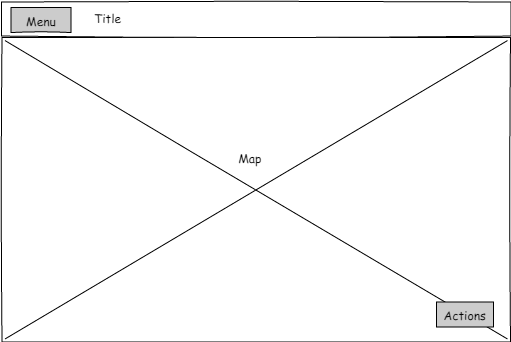
\includegraphics[width=0.7\linewidth]{startview.png}
\caption{Start Ansicht des Frontends}
\label{fig:startview}
\end{figure}

\begin{figure}
\centering
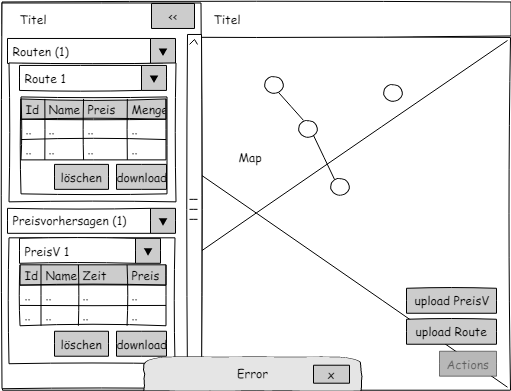
\includegraphics[width=0.7\linewidth]{draweropen.png}
\caption{Frontend während Verwendung}
\label{fig:draweropen}
\end{figure}

\subsection{Implementierung}

Zur Implementierung des Frontends wurde auf Web-Technologien gesetzt. Dies erlaubt eine kurze Feedback Loop bei der Entwicklung. Zur Entwicklung wurde die Sprache TypeScript verwendet. Bei TypeScript handelt es sich um ein Superset von Javascript, das um ein starkes Typsystem erweitert wurde. Durch die starke Typisierung ist es möglich, bereits während der Entwicklung Fehler zu erkennen, die bei der Verwendung von JavaScript erst zur Laufzeit auftreten.

Zu den nennenswerten eingesetzten Bibliotheken zählen OpenLayers 4 zur Darstellung von Karten, vue.js als Framework zur Erstellung von \acp{SPA} und vue-material als Komponenten Bibliothek.

Die Anwendung wurde in vue.js Komponenten unterteilt. Diese Komponenten befinden sich im Ordner \texttt{frontend/vue} und bestehen jeweils aus einer \texttt{.html} und einer \texttt{.ts} Datei. Die \texttt{.ts} Datei definiert das Verhalten der Komponente und die \texttt{.html} Datei das Aussehen.

Die Hauptkomponente, die die untergeordneten Komponenten instanziiert und für die Orchestration der Anwendung zuständig ist, befindet sich in den Dateien \texttt{index.ts} und \texttt{index-template.html}. Funktionalitäten, die nicht die Darstellung der Benutzeroberfläche beeinflussen, wurden im Ordner \texttt{frontend/app} abgelegt.

Die Darstellung der Karte verwenden OpenLayers 4. Die angezeigte Basiskarte ist von \ac{OSM} und erfordert eine aktive Internetverbindung während der Verwendung der Anwendung.

Während der Entwicklung der Anwendung kann der Webpack Dev Server mit dem Script \texttt{start} über das Tool yarn gestartet werden. Der Dev Server erstellt das Frontend nach Änderungen am Quellcode neu und triggert einen Reload des Browsers, falls nötig. Für die Auslieferung der Anwendung startet der Maven Build das Script \texttt{build} und kopiert die resultierenden Dateien in den Ordner \texttt{resources/public}. Spark ist so konfiguriert, dass der Inhalt dieses Ordners als statischer Inhalt zur Verfügung steht.

\subsection{Tests}

Für das Frontend wurden keine automatisierten Tests implementiert. Aufgrund der Überschaubarkeit der Anwendung wurde hierbei auf ein manuelles Testprotokoll zurückgegriffen. Das Testprotokoll beinhaltet folgende Schritte:

\begin{enumerate}
\item Frontend öffnen
\item Action Route Uploaden aufrufen
\item Prüfen, ob Karte auf Route zoomt
\item Prüfen, ob Ergebnis in seitlichem Menü angezeigt wird
\item Action Preisvorhersage Uploaden aufrufen
\item Prüfen, ob Karte auf angefragte Tankstellen zoomt
\item Prüfen, ob Ergebnis in seitlichem Menü angezeigt wird
\item Weitere Route hinzufügen
\item Erste Route löschen
\item Prüfen, ob erste Route nicht mehr in Ergebnisliste ist
\item Weitere Preisvorhersage hinzufügen
\item Erste Preisvorhersage löschen
\item Prüfen, ob erste Route nicht mehr in Ergebnisliste ist
\item Action Route Downloaden aufrufen
\item Prüfen, ob CSV korrekt ist
\item Action Preisvorhersage Downloaden aufrufen
\item Prüfen, ob CSV korrekt ist
\end{enumerate}

\subsection{Einschränkungen}

Während der Entwicklung wurde der aktuellste Chrome Browser von Google verwendet. Andere Browser werden momentan nicht unterstützt. Zum Zeitpunkt der Erstellung dieser Dokumentation, ist zumindest ein Bug in Firefox bekannt, der das Downloaden von Routen verhindert.



\section{Datenverarbeitung / Preisvorhersage} \label{feng}
In diesem Kapitel werden unsere Entscheidungen bezüglich der verwendeten Lernalgorithmen und der Datenverarbeitung dokumentiert. 
\subsection{Feature Engineering} 
Der erste Vorbereitungsschritt war, die vorhandenen Daten auf eine einheitliche Frequenz zu bringen. Um dies zu erreichen, wurde eine Datenbanktabelle mit stündlichen Zeitstempeln von Beginn der Aufzeichnung an bemustert. Anschließend wurde für jeden Zeitstempel ein Preis $p(t)$ nach folgendem Kriterium eingetragen:
\begin{equation*}
p(t) = \begin{cases}
p_{neu}, & \text{falls für } [t, t+1] \text{ ein neuer Preis $p_{neu}$ vorhanden ist}\\
p(t-1), & \text{sonst} 
\end{cases}
\end{equation*}

Dieses Grundgerüst eines Feature-Vektors wurde um die in \autoref{tab:features} aufgeführten zusätzlichen Merkmale erweitert. Durch die Persistierung der Daten in einer Datenbank kann effizient darauf zugegriffen werden. Bei den vorhandenen Datenmengen wäre ein Verbund mehrerer Datenbanktabellen zu zeitaufwendig, weshalb die redundante Speicherung mancher Daten in Kauf genommen wird. Für das Training des Regressionsalgorithmus wird aus dem Datensatz eine Trainingsmenge mit 75\% des gesamten Datensatzes erstellt. Die restlichen 25 \% ergeben die Testmenge zur Validierung unseres Modells.

\begin{table}
	\centering
	\begin{tabular}{l r}
		\textbf{Merkmal} & \textbf{Ursprung} \\ 
		\hline \hline
		Feiertage & \texttt{holidays} Python Package  \cite{holidays} \\ 
		Schulferien &  Schulferien.org \cite{ferien} \\ 
		Bundesland & 
        \multirow{3}{*}{ $\Bigg\}$ OpenStreetMap \cite{osm}}\\
        Landkreis &\\
        nächste Hauptverkehrsstraße & \\
		\hline 
	\end{tabular}
	\caption{Auflistung der zusätzlich verwendeten Merkmale pro Benzinpreis und Tankstelle.}
	\label{tab:features}	
\end{table} 

\subsubsection*{Feature Importance}
Mit dem eingesetzten Analysewerkzeug H2O können die für das Training verwendeten Features hinsichtlich ihrer Relevanz für die gegebene Problemstellung untersucht werden. Die Ergebnisse dieser Analyse sind in \autoref{fig:fi} grafisch dargestellt. Interessant ist hierbei, dass das Jahr der Messung das wichtigste Merkmal für die Vorhersage von Benzinpreisen darstellt. Diese Tatsache ist auf die heftige Schwankung des Benzinpreises in den letzten Jahren zurückzuführen. In \autoref{fig:bpe} sind die Jahresdurchschnittspreise für einen Liter Super Benzin der letzten 6 Jahre zu sehen. In dieser Grafik ist zu erkennen, dass der Benzinpreis im Jahr 2012 noch sehr hoch war, wohingegen er von 2014 bis 2016 stetig gesunken ist. Die Frankfurter Allgemeine Zeitung führt dies auf die geringe Nachfrage nach Rohöl in den Jahren 2014 und 2015 zurück, sowie auf die Einführung von Fracking in den USA, welche den Rohölpreis deutlich sinken ließ \cite{faz}. Jedoch ist auch die Tageszeit, die ID der entsprechenden Tankstelle und der Landkreis wichtig für die Vorhersage des Benzinpreises.
\begin{figure}
\centering
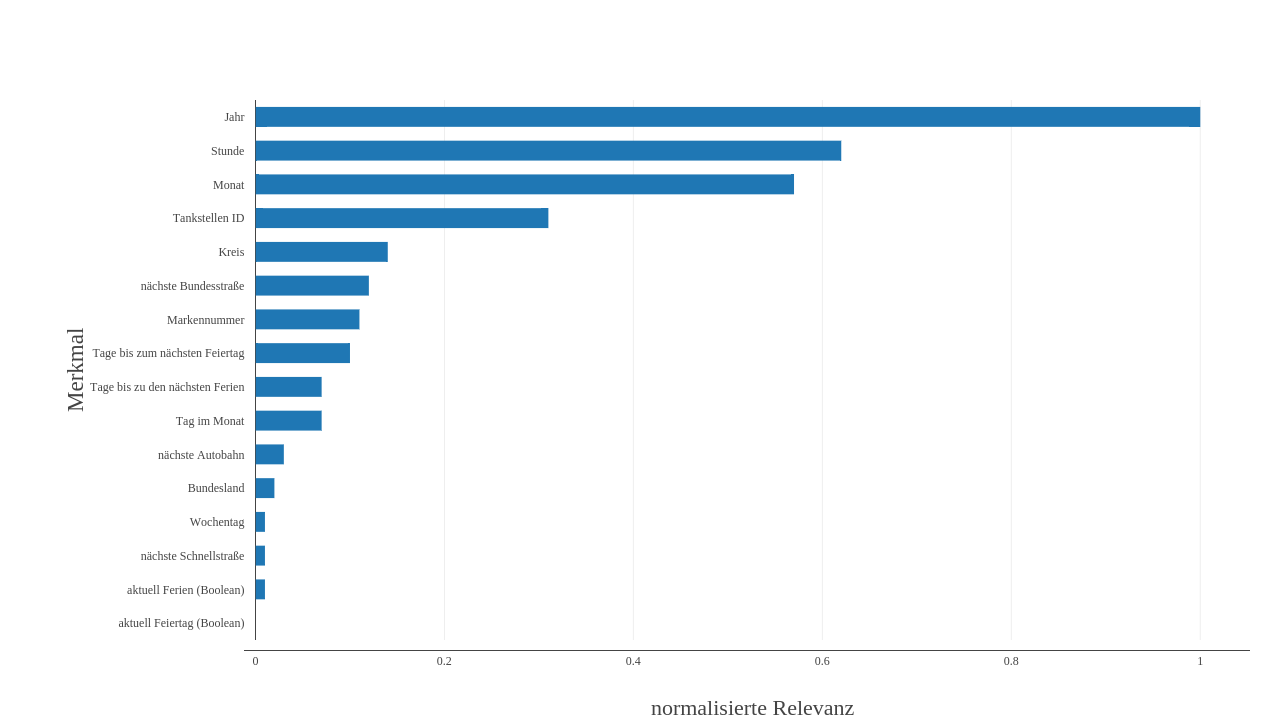
\includegraphics[width=\linewidth]{features720p.png}
\caption{Relative Relevanz der einzelnen Merkmale für die Vorhersage von Benzinpreisen.}
\label{fig:fi}
\end{figure}

\begin{figure}
\centering
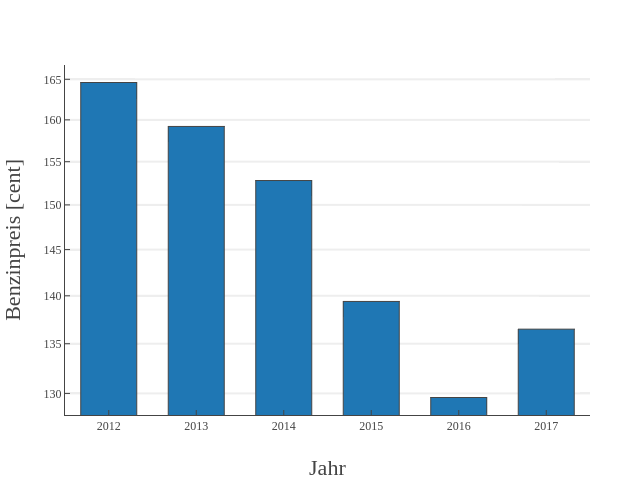
\includegraphics[width=0.7\linewidth]{Benzinpreisentwicklung_2012-2017.png}
\caption{Entwicklung der Jahresdurchschnittspreise für einen Liter Super Benzin in den Jahren 2012 bis 2017. Die Daten stammen von statista.com  \cite{stat}.}
\label{fig:bpe}
\end{figure}


\subsection{Modellauswahl}
Als erster Ansatz wurden unterschiedliche \ac{ARMA}-Modelle untersucht. Diese lassen jedoch keine Verwendung exogener Variablen zu, welche, wie später gezeigt, eine hohe Relevanz für die Vorhersage von Benzinpreisen besitzen. Anschließend wurden unterschiedliche maschinelle Lernverfahren untersucht, darunter auch einfache Deep-Learning Ansätze. Die manuelle Untersuchung dieser Algorithmen beansprucht jedoch viel Zeit. Um nicht unter Zeitdruck zu geraten, wurde die Modellsuche mit Hilfe der Open-Source Software H2O automatisiert. H2O implementiert Algorithmen aus den Bereichen Statistik, Data Mining und Maschinellem Lernen. Die Software basiert auf dem Hadoop Distributed File System, sodass ein Performance-Gewinn gegenüber anderen Analysewerkzeugen erzielt wird. \\
\par 
H2O kann mehrere Modelle des gleichen Typs mit anderen Modellen vergleichen und so das beste Modell für die gegebene Problemstellung finden. Durch ein Grid-Search werden die Hyperparameter der Modelle optimiert. Somit ist es möglich, in relativ kurzer Zeit ein wettbewerbsfähiges Modell zu erstellen. Für die gegebene Problemstellung hat sich ein \ac{GBM}-Modell als besonders potent herausgestellt. Die Eigenschaften dieses Modells werden nachfolgend kurz erläutert.

\subsubsection*{Gradient Boosting Machine}
Die Erklärung der \ac{GBM} erfolgt nach Friedmann \cite{gbm}. Durch Gradient Boosting wird ein Ensemble aus mehreren einfachen Modellen gebildet, welche als Aggregat ein neues und stärkeres Modell bilden. Die beinhalteten Modelle werden dabei so gebildet, dass der Gesamtfehler aller Modelle, inklusive des neu erstellten Modells, minimiert wird. Dies geschieht über den Gradienten der Fehlerfunktion unter Berücksichtigung der Vorhersage. Der Algorithmus funktioniert dabei wie folgt:

\begin{enumerate}
\item Ein Modell, üblicherweise ein Entscheidungsbaum, wird auf die Daten angepasst: 
\begin{equation*}
F_1(x) = y
\end{equation*}
\item Ein zweites Modell wird auf die Restwerte des ersten Modells angepasst:
\begin{equation*}
h_1(x) = y - F_1(x)
\end{equation*}
\item Aus diesen Modellen wird additiv ein neues Modell gebildet:
\begin{equation*}
F_2(x) = F_1(x) + h_1(x)
\end{equation*}
\end{enumerate}

Die grundlegende Idee dieses Boosting-Verfahrens ist es also, immer neue Modelle hinzuzufügen, die den Fehler des vorherigen Modells korrigieren. Das Modell wird über die Minimierung einer definierten Fehlerfunktion $L(y, F(x))$ trainiert. Diese Optimierung geschieht über ein Gradientenverfahren. Es ergeben sich folgende Aktualisierungsregeln:

\begin{equation*}
F_m(x) = F_{m-1}(x) - \gamma_m \sum_{i=1}^{n} \nabla_{F_m(x)} L(y_i, F_{m-1}(x_i))
\end{equation*}

Wobei $\gamma_m$ die Lernrate des aktuell betrachteten Modells repräsentiert. Diese Lernrate wird adaptiv nach folgender Vorschrift angepasst:

\begin{equation*}
\gamma_m = \argmin_\gamma \sum_{i=1}^{n} L\bigl(y_i, F_{m-1}(x) - \gamma \nabla_{F_m(x)} L(y_i, F_{m-1}(x_i))\bigr)
\end{equation*}

\subsubsection*{Ergebnisse der Grid Search}
Die Hyperparameter der implementierten GBM wurden durch eine Grid Search optimiert. \autoref{tab:params} gibt eine Übersicht über die wichtigsten Hyperparameter-Werte des Modells.

\begin{table}[h]
	\centering
	\begin{tabular}{l r}
		\textbf{Parameter} & \textbf{Wert} \\ 
		\hline \hline
		Anzahl an Entscheidungsbäumen & 50 \\ 
		Anzahl interner Bäume & 50  \\
		Minimale Tiefe & 5 \\
        Maximale Tiefe & 5\\
        Minimale Anzahl an Blättern & 32 \\
        Maximale Anzahl an Blättern & 32 \\
        K-fold cross validation & K=5 \\
        Lernrate & 0.1 \\
		\hline 
	\end{tabular}
	\caption{Die Hyperparameter-Werte des GBM-Modells, welche durch die Grid-Search optimiert wurden.}
	\label{tab:params}	
\end{table} 

\subsection{Training}
Da die ursprünglich als Zeitreihenvorhersage gedachte Aufgabenstellung durch eine Regressionsaufgabe substituiert werden konnte, trainiert das implementierte Modell mit dem gesamten Datensatz. Dies ist insbesondere für Preisvorhersagen, welche weit außerhalb der vorhandenen Datenbasis liegen von Vorteil. Der größte Nachteil an dieser Methode ist die benötigte Rechenpower. Die Trainingsmenge umfasst beinahe 15 Gigabyte. Da H2O den Datensatz komplett in den Arbeitsspeicher lädt, wird für das Training eine dementsprechend starke Rechenmaschine benötigt. Um dieses Modell zu trainieren, wurde daher auf eine Deep Learning Workstation mit 64 Gigabyte Arbeitsspeicher zurückgegriffen.\\
\par

\section{CLI}

Zum automatisierten Vergleich der Ergebnisse der Anwendung mit den Ergebnissen vergleichbarer Anwendungen wurde ein \ac{CLI} implementiert. Dieses \ac{CLI} benötigt Python 3.6 und ist im Unterordner \texttt{CLI} enthalten. Der Aufruf für die Berechnung einer Tankstrategie ist wie folgt:

\begin{lstlisting}
python cli.py --input pfad_zu_csv --output pfad_zu_output \
--host "http://localhost:4567" --type route
\end{lstlisting}

Für den Abruf einer Preisvorhersage kann Folgendes verwendet werden:

\begin{lstlisting}
python cli.py --input pfad_zu_csv --output pfad_zu_output \
--host "http://localhost:4567" --type pred
\end{lstlisting}

\chapter{Besonderheiten / Vorteile bei bestimmten Routen / Preisvorhersagen}

Dieses Kapitel geht auf Besonderheiten der Anwendung ein und schlägt Routen und Preisvorhersagen vor, die diese Besonderheiten hervorheben. Sämtliche vorgeschlagenen Routen und Preisvorhersagen sind im Ordner \path{routingService/src/test/resources/com/github/robinbaumann/informaticup2018} als \ac{CSV} Dateien enthalten. Die folgenden Abschnitte beschreiben jeweils in Tabellenform solche Daten.

Sämtliche hier beschriebenen Datensätze werden in den Integration Tests verwendet, um die Korrektheit des Verhaltens sicherzustellen.
\section{Fehlerfälle}
\subsection{Nicht existierende Tankstellen}

\begin{table}[H]
	\centering
	\begin{tabular}{l l}
		\textbf{Typ} &\textbf{Tankstrategie} \\
		\hline
		\hline 
		\textbf{Dateiname} & bertha\_bogus\_station.csv \\
        \textbf{Besonderheit} & enthält eine Tankstellen Id, die es nicht gibt \\
        \textbf{Verhalten} & Anwendung antwortet mit entsprechender ProblemResponse, kein Absturz \\
		\hline 
	\end{tabular}
\end{table} 

\subsection{Leere Tankstrategie}

\begin{table}[H]
	\centering
	\begin{tabular}{l l}
		\textbf{Typ} & \textbf{Tankstrategie} \\ 
		\hline
		\hline
		\textbf{Dateiname} & bertha\_empty.csv \\
        \textbf{Besonderheit} & enthält nur die Kapazität \\
        \textbf{Verhalten} & Anwendung antwortet mit entsprechender ProblemResponse, kein Absturz \\
		\hline 
	\end{tabular}
\end{table} 

\subsection{Negative Tankkapazität}

\begin{table}[H]
	\centering
	\begin{tabular}{l l}
		\textbf{Typ} & \textbf{Tankstrategie} \\
		\hline
		\hline 
		\textbf{Dateiname} & bertha\_negative\_capacity.csv \\
        \textbf{Besonderheit} & die Tankkapzität hat einen negativen Wert \\
        \textbf{Verhalten} & Anwendung antwortet mit entsprechender ProblemResponse, kein Absturz \\
		\hline 
	\end{tabular}
\end{table} 

\subsection{Tankstops sind nicht in zeitlicher Reihenfolge}

\begin{table}[H]
	\centering
	\begin{tabular}{l l}
		\textbf{Typ} & \textbf{Tankstrategie} \\
		\hline
		\hline
		\textbf{Dateiname} & bertha\_out\_of\_order.csv \\
        \textbf{Besonderheit} & zwei Tankstops wurden vertauscht, die Reihenfolge in der CSV \\
        & entspricht nicht der zeitlichen Reihenfolge \\
        \textbf{Verhalten} & Anwendung antwortet mit entsprechender ProblemResponse, kein Absturz \\
		\hline 
	\end{tabular}
\end{table} 

\subsection{Routen mit Tankstellen ohne Preisinformationen}

\begin{table}[H]
	\centering
	\begin{tabular}{l l}
		\textbf{Typ} & \textbf{Tankstrategie} \\ 
		\hline
		\hline
		\textbf{Dateiname} & bertha\_stations\_without\_prices.csv \\
        \textbf{Besonderheit} & Es werden Tankstellen angefragt für die in den Originaldaten \\ 
        & keine Preise hinterlegt waren \\
        \textbf{Verhalten} & Anwendung antwortet mit entsprechender ProblemResponse, kein Absturz \\
		\hline 
	\end{tabular}
\end{table} 

\subsection{Daten nach angefragtem Zeitpunkt verfügbar}

\begin{table}[H]
	\centering
	\begin{tabular}{l p{12cm}}
		\textbf{Typ} & \textbf{Preisvorhersage} \\ 
		\hline
		\hline
		\textbf{Dateiname} & price-prediction-historic.csv \\
        \textbf{Besonderheit} & Es wird ein Preis angefragt und es können Daten bis nach dem angefragten Zeitpunkt \\
        & verwendet werden \\
        \textbf{Verhalten} & Anwendung antwortet mit dem tatsächlichen Preis zu dem Zeitpunkt \\
		\hline 
	\end{tabular}
\end{table} 


\subsection{Daten bis kurz vor angefragtem Zeitpunkt verfügbar}

\begin{table}[H]
	\centering
	\begin{tabular}{l l}
		\textbf{Typ} & \textbf{Preisvorhersage} \\ 
		\hline
		\hline
		\textbf{Dateiname} & price-prediction-very-close.csv \\
        \textbf{Besonderheit} & Es wird ein Preis angefragt und es können Daten bis kurz vor (1h) dem \\
        & angefragten Zeitpunkt verwendet werden \\
        \textbf{Verhalten} & Anwendung antwortet letztem tatsächlichen Preis zu dem Zeitpunkt \\
		\hline 
	\end{tabular}
\end{table} 

\subsection{Routen Stops nicht erreichbar mit vollem Tank}

\begin{table}[H]
	\centering
	\begin{tabular}{l p{12cm}}
		\textbf{Typ} & \textbf{Tankstrategie} \\ 
		\hline
		\hline
		\textbf{Dateiname} & not-reachable.csv \\
        \textbf{Besonderheit} & An einer gewissen Position in der Route, ist der nächste Stopp selbst mit vollem Tank nicht erreichbar. \\
        \textbf{Verhalten} & Anwendung antwortet mit entsprechender ProblemResponse, kein Absturz \\
		\hline 
	\end{tabular}
\end{table} 
\section{Fehlversuche}

Unser hinreichend gutes Ergebnis mittels der 'Gradient Boosting Machine' auf dem Framework 'h2o' ist Ergebnis einer umfangreichen 'Data-Exploration': Es wurden verschiedene Modelle und Algorithmen verglichen um ein Vorhersagemodell zu entwerfen. Unsere Vorgehensweise war allgemein wie folgt:

\begin{description}
	\item[Daten-Präparation]
Die Angleichung und Vorverarbeitung von den Features (auch Feature-Engineering genannt).
	\item[Modellerstellung] 
	Die Erstellung und Bewertung verschiedener Modelle und Algorithmen für unsere Domäne.
\end{description}

Während dieses Prozesses, wurden häufig Modelle und Algorithmen verworfen. Einige werden in diesem Kapitel dargelegt und begründet, wieso sie nicht zu unserem Problem passten.

\subsection{Daten-Präparation}

Während der Daten-Präparation zum Testen einiger Modelle, genügte es häufig ein Bruchteil des gesamten Datensatzes zum Trainieren zu verwenden und wiederum ein Bruchteil dessen, um es zu testen.
Viele Modelle benötigten eine stationäre Zeitserie an Daten.
Damit ist gemeint, dass jeglicher Datenpunkt in der Serie unabhängig von der Zeit ist.\\
Anfänglich lagen unsere Daten von unterschiedlichen Tankstellen zu unterschiedlichsten Messzeiten vor. Modelle wie 'ARIMA' benötigen eine gleichbleibende Frequenz der Daten-Zeitpunkte. Also wurden die Daten in eine einheitliche Frequenz abgetastet. Mit Hilfe von PostGreSQL konnten wir die Daten nun zu stündlichen Messpunkten vorlegen. 
Üblicherweise werden diese Daten von einem 'Trend' und 'Saisonalität' bereinigt.\\
Um die Stationärität eines Datensatzes zu bewerten wird häufig der 'Augmented Dickey–Fuller test' \cite{stationarity} und zur Bereinigung der Daten hierfür verschiedene Methoden wie die Daten zu logarithmieren oder mittels 'First order Difference' (Differenz der Zeitserie mit nach der um $t$ Zeitpunkten verschobenen Zeitserie) angewendet. 
Mittels unseres anfänglichen bereinigten Datensatzes, war es uns nun möglich eine 'Partial Autocorrelation'\cite{pacf} (ähnlich wie bei ARIMA) durchzuführen. Dadurch wird ein Korrelationskoeffizient berechnet, welcher aussagt, wie sehr eine um $t$ Zeitpunkten verschobene Zeitreihe verglichen zu sich selbst, korreliert.\\
Als Ergebnis für verschiedene 'Time-Lags' schlossen wir dass die Zeitreihe nach einem 'lag' am meisten mit sich selbst korreliert, also der Benzinpreis einer Stunde vorher am meisten darüber aussagen kann, wie sich der Benzinpreis in einer Stunde entwickeln wird.
Dadurch, dass wir die Benzinpreise stündlich abtasteten lag es Nahe, dass der vorhergehende Preis nicht nur ähnlich ist, sogar sehr wahrscheinlich derselbe. Denn falls zu einem Zeitpunkt $t_k$ kein neuer Preis vorliegt, wird der von $t_{k-1}$ übernommen.

\subsection{Modellerstellung}

Durch unsere fälschliche Annahme durch die partielle Autokorrelation, entwarfen wir ein Modell mit Hilfe der 'Linearen Regression'.
Das erste Modell wies eine vorhergesagte Zeitreihe mit einem extremen Trend und starker Abweichung der tatsächlichen Daten vor (Underfitting). Somit wurde das Modell modifiziert und zur 'Lasso-Regression' überführt.

$$ \sum_{i}^{n}(y_i - \sum_{j}^{m} x_{ij}\beta_j)^2 + \lambda \sum_{1}^{p} |\beta_j| $$

Die oben genannte Formel gilt es zu minimieren.
Durch die Lasso-Regression wird eine sogenannte L1-Regulation angewendet. Durch zu große Gewichtungsfaktoren $\beta_k$ wird das Ergebnis insgesamt größer, da $\beta$ zusätzlich als 'Strafwert' dazu addiert wird. Dadurch werden beim Trainieren automatisch die Features stärker gewichtet, welche größeren Einfluss auf das gesamt Ergebnis haben (vice versa gilt: Features die wenig oder keinen Einfluss haben werden vernachlässigt).\\
Das Ergebnis der Lasso-Regression war überraschend gut, jedoch war es uns nur möglich Preise eine Stunde vorauszusagen (One-Step-Ahead-Forecast). Die Aufgabenstellung erwartete jedoch eine Vorhersage für bis zu einem Monat. Es wäre zwar möglich gewesen das Modell mehrmals auf sich selbst anzuwenden ( $f(x_0) \circ f(x_1) \circ f(x_2) \circ ... $ (Multi-Step-Forecast)), dadurch würde jedoch jeder Fehler, je öfter das Modell mit sich selbst angewendet wird, stärker gewichtet.\\
\begin{figure}
	\centering
	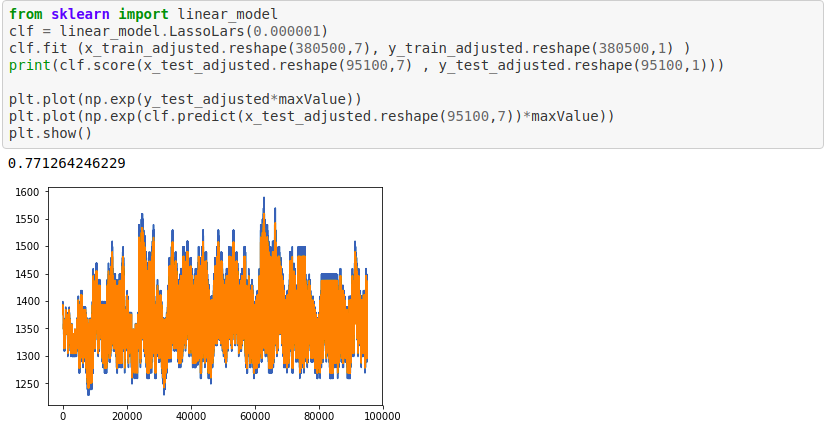
\includegraphics[width=0.7\linewidth]{images/fehlversuch}
	\caption{Die tatsächlichen Preise (orange) und die der Lasso-Regression vorhergesagten (blau und von der orangefarbenen Kurve verdeckt)}
	\label{fig:fehlversuch}
\end{figure}
In Abbildung \ref{fig:fehlversuch} ist die Bewertung der Lasso-Regression zu sehen. Die orangefarbenen Werte sind die tatsächlichen Werte der Tankstellen. Es wurden 100.000 Datenpunkte zum Testen verwendet. Auf der Y-Achse sind die Preise von $1,25$ Euro bis $1,60$ Euro pro Liter zu sehen. Die orangefarbene Kurve verdeckt die vorhergesagten blauen Werte, welche nur teilweise ein höheres bzw. niedrigeres Ergebnis lieferten, sich aber ansonsten deckten. Das Framework 'sklearn' bewertet das Modell mit 77 Prozent.
Dieser Score setzt sich aus den summierten Differenzen der tatsächlichen Preisen und den vorhergesagten Preisen, geteilt durch die Anzahl der Beobachtungspunkte zusammen.\\
Neben der Lasso-Regression wurde auch ARIMA getestet, da wir in diesem Modell aber keine zusätzlichen Features außer Zeitpunkt und Benzinpreis (zwei dimensional) einbringen konnten, wurde dies sehr schnell verworfen.


\section{Evaluation}
In diesem Abschnitt wird die allgemeine Vorhersagegüte des erstellten Modells zur Benzinpreisvorhersage diskutiert.

\subsection{Fixed-Path-Gas-Station Algorithmus}
Zusätzlich zu den im vorherigen Abschnitt genannten Routen wurden noch vier weitere zur Evaluierung der hier implementierten Tankstrategie gegen die oben definierte naive Tankstrategie erstellt. Es werden nun vier Routen verglichen anhand der tatsächlichen Kosten, die nach den zwei Tankstrategien jeweils anfallen würden. Die Euro-Beträge sind auf die zweite Dezimalstelle und die Prozentwerte auf eine ganze Zahl gerundet.

\begin{table}[H]
	\centering
	\begin{tabular}{l l}
		\textbf{Typ} & \textbf{Tankstrategie} \\ 
		\hline
		\hline
		\textbf{Dateiname} & test1.csv \\
        \textbf{Naive Strategie} & 50.96\euro{} \\
        \textbf{Optimale Strategie} & 25.70\euro{} \\
  		\textbf{Günstiger} & 25.26\euro{} \\
        \textbf{\% günstiger} & 50\% \\
		\hline 
	\end{tabular}
\end{table} 

\begin{table}[H]
	\centering
	\begin{tabular}{l l}
		\textbf{Typ} & \textbf{Tankstrategie} \\ 
		\hline
		\hline
		\textbf{Dateiname} & test2.csv \\
        \textbf{Naive Strategie} & 138.08\euro{} \\
        \textbf{Optimale Strategie} & 56.02\euro{} \\
  		\textbf{Günstiger} & 82.06\euro{} \\
        \textbf{\% günstiger} & 40\% \\
		\hline 
	\end{tabular}
\end{table} 

\begin{table}[H]
	\centering
	\begin{tabular}{l l}
		\textbf{Typ} & \textbf{Tankstrategie} \\ 
		\hline
		\hline
		\textbf{Dateiname} & test3.csv \\
        \textbf{Naive Strategie} & 118.01\euro{} \\
        \textbf{Optimale Strategie} & 68.17\euro{} \\
  		\textbf{Günstiger} & 49.84\euro{} \\
        \textbf{\% günstiger} & 57\% \\
		\hline 
	\end{tabular}
\end{table} 

\begin{table}[H]
	\centering
	\begin{tabular}{l l}
		\textbf{Typ} & \textbf{Tankstrategie} \\ 
		\hline
		\hline
		\textbf{Dateiname} & test4.csv \\
        \textbf{Naive Strategie} & 46.36\euro{} \\
        \textbf{Optimale Strategie} & 28.08\euro{} \\
  		\textbf{Differenz} & 18.28\euro{} \\
        \textbf{\% günstiger} & 60\% \\
		\hline 
	\end{tabular}
\end{table} 

Im Schnitt ist bei unseren vier Testversuchen die optimale Tankstrategie 51.75\% günstiger als die naive.

\subsection{Allgemeine Vorhersagegüte des Modells}

Um die allgemeine Vorhersagegüte des erstellten Modells diskutieren zu können, müssen zunächst die einzelnen Fehlermaße erläutert werden. Dies ist mit folgender Übersicht gegeben, wobei die Definitionen an \cite{maermse} angelehnt sind ($n$ := Anzahl der Vorhersagewerte, $\hat{y}_i$ := Vorhersagewerte, $y_i$ := Beobachtungswerte):

\newpage
\begin{itemize}
	\item \textbf{\acf{MAE}}: 
	\begin{itemize}
		\item Mathematische Definition: $MAE = \frac{1}{n} \sum_{i=1}^{n}|y_i - \hat{y}_i|$
		\item Der \ac{MAE} ist ein größenabhängiges Fehlermaß, der die mittlere absolute Abweichung von der Grundwahrheit ermittelt. 
	\end{itemize}
	\item \textbf{\acf{RMSE}}:
	\begin{itemize}
		\item Mathematische Definition: $RMSE = \sqrt{\frac{1}{n} \sum_{i=1}^{n}(y_i - \hat{y}_i)^2} $
		\item Der \ac{RMSE} gewichtet im Gegensatz zum \ac{MAE} die Größe der einzelnen Abweichungen durch Quadrierung. Für einen gleichmäßig verteilten Fehler sind beide Fehlermaße gleich, einzelne Ausreißer werden jedoch durch den \ac{RMSE} stärker gewichtet.
	\end{itemize}
	\item \textbf{Bestimmtheitsmaß $R^2$}:
	\begin{itemize}
		\item Mathematische Definition: $ R^2 = \frac{\sum_{i=1}^{n} (\hat{y}_i - \bar{y}_i)^2}{\sum_{i=1}^{n} (y_i - \bar{y}_i)^2}$
		\item Das Bestimmtheitsmaß liegt im Wertebereich [0,1] und ist ein Maß für die Anpassungsgüte einer Regression. Es beschreibt, wie viel Variation in den Daten durch das verwendete Regressionsmodell erklärt werden kann. 
	\end{itemize}
\end{itemize}

\begin{table}
	\centering
	\begin{tabular}{l l}
		\textbf{Fehlermaß} & \textbf{Wert} \\ 
		\hline 
		\hline
		\ac{MAE} & 2.98 cent/Liter \\ 
		\ac{RMSE} & 4.24 cent/Liter \\ 
		$R^2$ & 78.12 \% \\ 
		\hline
	\end{tabular} 
	\caption{Vergleich der drei Kennzahlen MAE, RMSE und $R^2$}
	\label{tab:eval}
\end{table}

Mit diesen Definitionen kann nun die Allgemeine Vorhersagegüte des erstellten Modells bewertet werden. In \autoref{tab:eval} sind die für das erstellte Modell berechneten Werte der jeweiligen Kennzahlen eingetragen. Zunächst sind die beiden Fehlermaße \ac{MAE} und \ac{RMSE} zu vergleichen. Für beide Fehlermaße gilt, dass niedrigere Werte besser sind. Desweiteren beschreiben beide Maße den durchschnittlichen Vorhersagefehler des Modells. Der Unterschied liegt in der Gewichtung der einzelnen Fehler. Beim \ac{RMSE} werden die Fehler vor der Mittelung quadriert. Dies ruft eine stärkere Gewichtung von Ausreißern hervor. Zu beachten ist, dass der \ac{RMSE} nicht mit der Varianz der Fehlerwerte steigt, sondern vielmehr mit der Varianz der Häufigkeitsverteilung der Fehlergrößen \cite{maermse}. Aus diesen Eigenschaften der Fehlermaße kann nun interpretiert werden, dass das erstellte Modell nicht für alle Tankstellen gleich gute Vorhersagen liefert. Dies ist daran zu erkennen, dass der \ac{RMSE} höher als der \ac{MAE} ist. Wenn für jede Vorhersage der gleiche Fehler entstünde, besäßen die beiden Fehlermaße den gleichen Wert. Eine Erklärung für die einzelnen Ausreißer ist, dass im Datensatz einige Tankstellen mit Lücken in den historischen Preisen existieren. Diese Lücken wurden durch das in Abschnitt \ref{feng} erläuterte Sampling der Preise auf eine stündliche Basis gefüllt. Dies ist ein Fehler, denn das Modell inhärent mitlernt. Es wäre zu untersuchen, ob eine Elimination dieser Tankstellen die Vorhersagegüte positiv beeinflusst. Jedoch bedeutet der Verzicht auf diese Tankstellen eine Verkleinerung des Datensatzes. \\
\par 
Der $R^2$-Wert von 78.12\% beschreibt eine gute Anpassung der Regression. Die gewählten erklärenden Variablen eignen sich also gut um die abhängige Variable zu beschreiben. Anders formuliert können durch das erstellte Modell 78.12\% der Varianz im Benzinpreis durch die gewählten erklärenden Variablen des Merkmalvektors beschrieben werden. \\
\par 

\begin{figure}
	\centering
	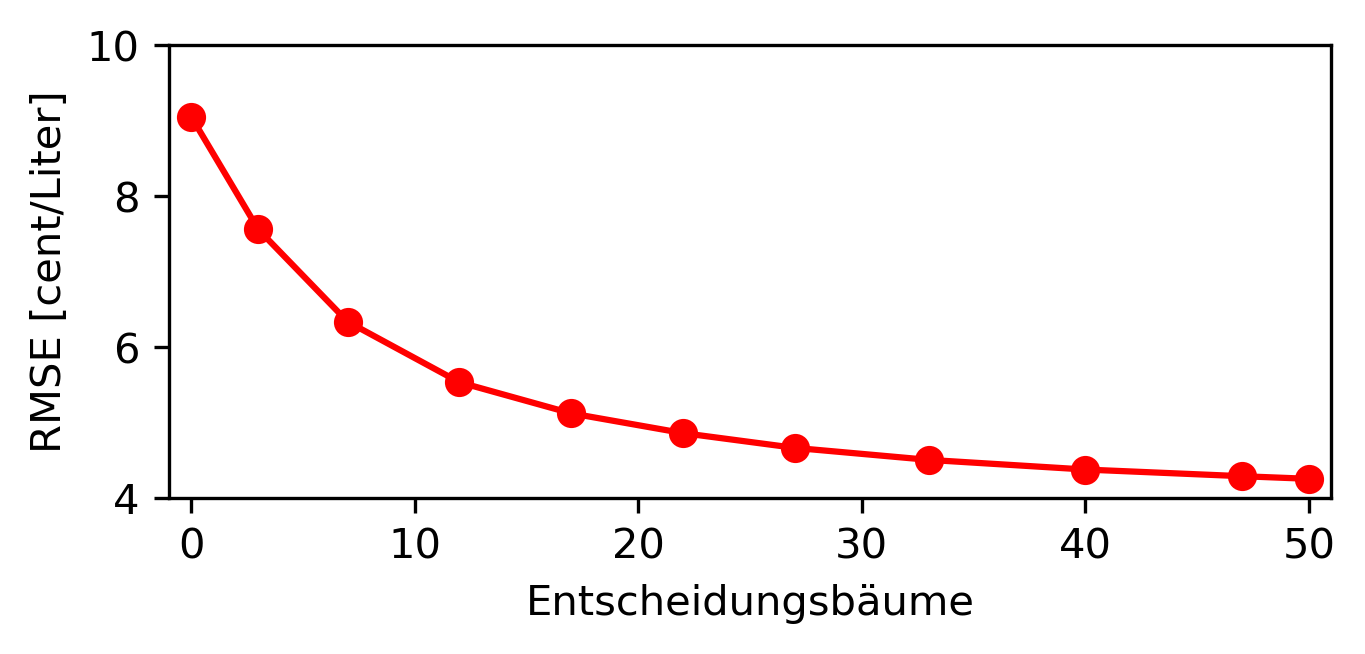
\includegraphics[width=0.7\linewidth]{images/eval_rmse_per_trees}
	\caption{RMSE pro Anzahl trainierter Entscheidungsbäume}
	\label{fig:evalrmsepertrees}
\end{figure}


In \autoref{fig:evalrmsepertrees} wird der \ac{RMSE} während des Trainings der \acl{GBM} aufgezeichnet. Es ist zu sehen, wie der Fehler bei fortschreitendem Training, also der Hinzunahme weiterer Entscheidungsbäume immer kleiner wird. Mit 50 Entscheidungsbäumen ist der finale \ac{RMSE} aus \autoref{tab:eval} erreicht. \\
\par 

Allgemein kann gesagt werden, dass das erstellte Modell eine gute Vorhersagegüte besitzt. Es können ungefähr 78 \% der Varianz in der Ergebnisvorhersage erklärt werden. Da das erstellte Modell die Preise zu einem gegebenen Zeitpunkt direkt vorhersagen kann, also ohne direkte Abhängigkeit des in der Zeitreihe vorherigen Preises, wirkt der mittlere Fehler noch attraktiver. Das Modell kann somit nämlich auch Preise zuverlässig vorhersagen, die weiter als einen Monat in der Zukunft liegen. Für sehr weit in der Zukunft liegende Preisvorhersagen muss die letzte Aussage jedoch mit Vorsicht genossen werden, da der aktuelle Trend der Zeitreihe nicht garantiert die gleiche Steigung behält. Als Beispiel sei hier nochmals an den Preissturz im Jahr 2015 durch die Einführung des Frackings in den USA erinnert. Solche Ereignisse in der Zukunft können nur schwer vorhergesagt werden und erfordern deshalb eine regelmäßige Aktualisierung des Modells. Durch die direkte Vorhersage der Preise ergibt sich in diesem Modell ein Performance-Vorteil gegenüber schrittweisen Preisvorhersagen. Diese müssen nämlich für jede Preisvorhersage die aktuellsten Preise mit in die Berechnung einbeziehen, wohingegen das hier vorgestellte Modell direkt aus den gegeben Metadaten einen Preis für einen beliebigen Zeitpunkt berechnen kann. Der benötigte Aufwand zur regelmäßigen Aktualisierung des Modells wird hierbei in den Hintergrund verschoben, so dass der Endnutzer des Systems keine Verzögerungen in der Preisvorhersage erwarten muss. Zusammen mit den guten Ergebnissen des mittleren Fehlers von ca. 3 Cent/Liter kann von einer sehr guten Lösung der IntelliTank-Aufgabe gesprochen werden.


\chapter{Anwendungsszenario}
\label{sec:orgeeaadfe}
Die im Rahmen der Studienarbeit implementierte Anwendung stellt ein \ac{POC} dar. Es wurden einige Annahmen getroffen, die die Anwendung für den Einsatz unter realen Bedingungen ungeeignet machen. So erwartet die Anwendung eine Route als Eingabe, die aus einzelnen Tankstellen, sowie der Ankunftszeit an diesen Tankstellen besteht. Auch wurde keine Rücksicht darauf genommen, dass sich die Daten, die der Preisberechnung zugrunde liegen ständig ändern. Dieses Kapitel ist ein Gedankenexperiment, um die Schritte aufzuzeigen, die im Falle einer realen Verwendung der Anwendung nötig wären. Um dies zu erreichen wird zuerst ein reales Einsatzszenario definiert und anschließend werden die erforderlichen Schritte näher erläutert.

\section{Definition des Szenarios}
\label{sec:orge2ccbc7}
Es ist recht unrealistisch, dass ein Benutzer Autoreisen plant indem er sämtliche Tankstellen entlang seiner Route ermittelt und die jeweilige Ankunftszeit an den Tankstellen berechnet. Eine bessere \ac{UX} wäre es die Kalenderdaten des Benutzers abzufragen. Auf Basis der Termine im Kalender kann eine optimale Route berechnet werden.

Es wird die Annahme getroffen, dass die Termine im Kalender jeweils mit einer Adresse versehen sind und dass die Strecke von Termin zu Termin jeweils mit dem Auto bewältigt wird. Die Anwendung könnte so die optimale Route und Tankstrategie für einen gewissen Planungshorizont berechnen.

Dieser Anwendungsfall könnte auch von Privatpersonen auf Speditionen übertragen werden, um die Treibstoffkosten im Güterverkehr zu senken.

\section{Anpassung des Algorithmus}
\label{sec:org182565e}
Damit die Anwendung für dieses Szenario geeignet ist, müssen mehrere Teile angepasst werden. Die Anwendung verwendet bereits \ac{OSM} Daten, um weitere Features für die einzelnen Tankstellen zu ermitteln. Momentan werden hierfür lediglich Daten für Autobahnen, Schnell- und Bundesstraßen, Landes- und Kreisgrenzen verwendet. Diese Daten reichen für die erweiterten Anforderungen des Szenarios nicht aus.

Um die Routen zwischen den einzelnen Terminen zu ermitteln kann \emph{PostgreSQL/PostGIS} durch \emph{pgRouting} \footnote{\url{http://www.pgrouting.org}} erweitert werden. Diese Erweiterung benötigt als Grundlage einen gewichteten Graphen. Dieser Graph kann aus \ac{OSM}-Daten erstellt werden.

Um eine Route zu ermitteln benötigt \emph{pgRouting} jeweils die Id des Start- und Endknoten des Graphen. Deshalb muss es möglich sein von \ac{OSM}-Geometrien auf die entsprechende Id des Knoten zu schließen. Da der Benutzer seine Route anhand von Adressen in das System eingibt müssen diese zuerst in Geokoordinaten umgewandelt werden. Dieser Vorgang nennt sich \emph{reverse geocoding} und ist auch auf Basis von \ac{OSM}-Daten möglich. Dazu kann die Software \emph{Nominatim} \footnote{\url{http://www.nominatim.org}} verwendet werden. Die Geokoordinaten der Adresse genügen zur Ermittlung der Ids jedoch noch nicht. In einem weiteren Schritt muss die nächste Geometrie, die eine Repräsentierung im Graphen besitzt, ermittelt werden. Zur Beschleunigung dieser Query empfiehlt sich der Einsatz eines spatial index.

Um den Suchraum für die Route einzuschränken, empfiehlt es sich nur einen Teil des Graphen auszuwerten. Dies kann erreicht werden indem nur Knoten und Kanten verwendet werden, deren Geometrie innerhalb einer Bounding Box liegen. Eine einfache Lösung zur Ermittlung der Bounding Box wäre es die Koordinaten des Start- und Endpunktes zu ermitteln und ein Rechteck um diese zu legen und anschließend um einen Puffer zu erweitern.

Nachdem die optimale Route zwischen den Terminen ermittelt wurde geht es im nächsten Schritt darum Tankstellen entlang dieser Route zu finden. Die Route besteht aus Kanten des gewichteten Graphen und muss zuerst wieder in eine Geometrie übersetzt werden. Mit dieser Geometrie ist es möglich Tankstellen in einer gewissen Entfernung über einen Join der Tankstellen Tabelle zu ermitteln. Die gewünschte maximale Entfernung kann dabei im Join-Prädikat angegeben werden.

Im nächsten Schritt werden für die Tankstellen die entsprechenden Knoten der Routing-Datenbasis ermittelt. Es kann sein, dass diese Knoten noch nicht im Subgraphen, der für die Ermittlung der Route verwendet wurde enthalten sind. In diesem Fall muss der Subgraph erweitert werden. Mit diesen Daten kann nun die zu erwartende Ankunftszeit an den Tankstellen ermittelt werden. Über die Ankunftszeit kann anschließend der Preis vorhergesagt werden.

Der Graph mit der Route, Tankstellen und Preisen kann anschließend ausgewertet werden, um eine optimale Tankstrategie zu ermitteln. Dazu kann der Algorithmus von Lin \cite{transnet} verwendet werden. Der Algorithmus weist eine Zeitkomplexität von \(O(n^3)\) auf, wobei \(n\) die Anzahl an Knoten im Graphen bezeichnet. Dies kann bei langen Routen zu einer sehr hohen Laufzeit führen. Es wäre zu prüfen, ob eine Optimierung durch die Verwendung von evolutionären Algorithmen zu schnelleren Ergebnissen ähnlicher Güte führt.

Im nächsten Abschnitt wird aufgezeigt welche Daten für den angepassten Algorithmus verwendet werden und wie diese aktuell gehalten werden können

\section{Neuberechnung des Routing Graphen}
\label{sec:org520d5e2}
Zur Berechnung der optimalen Route werden die \ac{OSM}-Daten Deutschlands benötigt. Damit \emph{pgRouting} mit den Daten umgehen kann müssen sie in einen gewichteten Graphen umgewandelt werden. Dies kann mit der Funktion \texttt{pgr\_createTopology} erledigt werden. Abbildung \ref{fig:osminitial} veranschaulicht diesen Vorgang.

\begin{figure}[htbp]
\centering
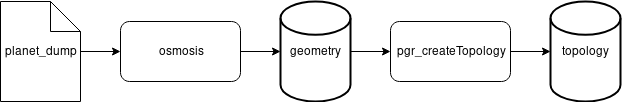
\includegraphics[width=.9\linewidth]{osm-data-initial.png}
\caption{\label{fig:orgfade148}
Initiales Laden von OSM Daten in die Datenbank und Erstellung eines gewichteten Graphen zur Routenberechnung}
\end{figure}

Die \ac{OSM}-Daten können inkrementell geupdatet werden. Hierzu stellt \ac{OSM} sogenannte \emph{change sets} zur Verfügung. Diese \emph{changesets} können mit einem Werkzeug wie \emph{osmosis} \footnote{\url{https://wiki.openstreetmap.org/wiki/Osmosis}} in die Datenbank eingelesen werden. Der gewichtete Graph muss bei jeder Änderung der Ursprungsdaten komplett neu berechnet werden.

Die \emph{changesets} sind zum Beispiel als \ac{XML}-Dateien mit einer minütlichen Auflösung erhältlich. Da eine minütliche Neuberechnung des gewichteten Graphen nicht praktikabel erscheint, können die \emph{changesets} gesammelt und in einem täglichen oder wöchentlichen Intervall aufgespielt werden. Dieser Vorgang wird in Abbildung \ref{fig:osmdata} gezeigt. Die \emph{changesets} werden im \emph{changeset buffer} zwischengespeichert. Täglich oder wöchentlich werden sie mit \emph{Osmosis} in die Geometrie-Tabelle übernommen. Daraufhin wird der \emph{changeset buffer} geleert und der gewichtete Graph wird durch \texttt{pgr\_createTopology} neu erstellt. Der Parameter \texttt{clean} sorgt dafür, dass die entsprechende Tabelle davor geleert wird.

\begin{figure}[htbp]
\centering
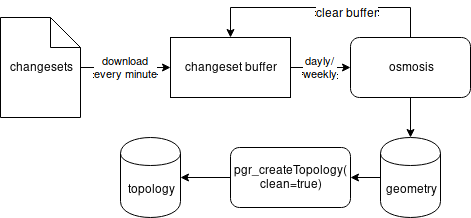
\includegraphics[width=.9\linewidth]{osm-data-update.png}
\caption{\label{fig:orgbb24e88}
Update der OSM Geometrien und Neuberechnung des gewichteten Graphen}
\end{figure}

Neben den Daten für die Berechnung der Route werden noch die Preise für die Ermittlung der Tankstrategie benötigt. Der nächste Abschnitt bestimmt welche Daten dies betrifft und wie mit Änderungen an diesen Daten umgegangen wird.
\section{Neuberechnung des Modells zur Preisvorhersage}
\label{sec:org2499f4b}
Die historischen Benzinpreise der Tankstellen wurden mit Informationen zu Feiertagen, Schulferien Bundesland, Landkreis und den nächsten Hauptverkehrsstraßen erweitert. Mit diesen erweiterten Daten benötigte das Training der \ac{GBM} über die historischen Daten in etwa 3 Stunden. Zum Training wurde ein Rechner mit einem AMD Threadripper 1950x, 64GB Arbeitsspeicher und einem SSD-Hintergrundspeicher verwendet.

Nach dem Training kann das Modell in Form einer Zip-Datei aus H2O extrahiert werden. Diese Zip-Datei wird zur Laufzeit in die Anwendung geladen und zur Vorhersage der Benzinpreise verwendet. Um immer die aktuellsten Entwicklungen auf dem Benzinmarkt zu berücksichtigen, sollte das Modell in regelmäßigen Zeitabständen neu trainiert werden. Dieser Vorgang kann losgelöst von der eigentlichen Anwendung ablaufen.

Die historischen Benzinpreise bestehen aus zwei Tabellen. Den Preisen an sich und Informationen zu den einzelnen Tankstellen. Dabei sind nicht alle Spalten der Tabellen für die Vorhersage relevant. Aus der Tabelle Preise wird das Datum, der Preis und die Id der Tankstelle benötigt. Über die Id wird die Tabelle Tankstellen mit den Preisen verbunden. Hier sind neben der Marke noch die Koordinaten der Tankstelle, also Latitude und Longitude, relevant.

Im nächsten Schritt wird das Datum der Preise in die Komponenten Jahr, Monat, Tag der Woche, Stunde und Tag des Monats zerlegt. Auf Basis der Koordinaten wird jeweils für die unterschiedlichen Arten an Hauptverkehrsstraßen ermittelt welche Hauptverkehrsstraße den geringsten Abstand zur Tankstelle hat. Dabei werden nur Hauptverkehrsstraßen innerhalb von 5 Km betrachtet. Auch auf Basis der Koordinaten wird das Bundesland und der Landkreis der Tankstelle ermittelt.

Nach der Aufbereitung der Daten kann letztendlich das Modell trainiert werden. Beim Erhalt von neuen Benzinpreisen muss nur das Datum zerlegt werden, da die Informationen zu den Tankstellen bereits vorliegen. Falls eine unbekannte Tankstelle in den Daten erscheint, werden die dazugehörigen Informationen für die Tankstelle berechnet und gespeichert.

Nach der Identifikation der sich ändernden und benötigten Daten kann eine Strategie entwickelt werden um die Anwendung für die Verwendung durch viele Benutzer zu skalieren. Diese Strategie wird im nächsten Abschnitt behandelt.
\section{Entwicklung einer Architektur zur Skalierung der Anwendung}
\label{sec:orgcd082c3}
Bereits bei der Entwicklung der \ac{POC} Version der Anwendung wurde darauf geachtet, dass die einzelnen Anfragen keine Nebeneffekte verursachen. In der Praxis bedeutet dies, dass eine Anfrage nicht den Zustand der Anwendung verändert. Das wird dadurch erreicht, dass die Anwendung nur lesend auf die Daten zugreift.

Dadurch ist es möglich die Anwendung horizontal zu skalieren. Horizontale Skalierung bedeutet, dass die maximale Anzahl gleichzeitiger Anfragen gesteigert werden kann, indem mehr Rechner dem System hinzugefügt werden.

Abbildung \ref{fig:scaling} zeigt eine mögliche Architektur, die diesen Sachverhalt ausnutzt, um die Anwendung für viele Anwender gleichzeitig nutzbar zu machen. Das System wird in die zwei Zonen "blue" und "green" unterteilt. Es ist jeweils nur eine der Zonen gleichzeitig aktiv. Eine Anfrage eines Benutzers zur Berechnung einer optimalen Route (\texttt{RoutingRequest}) wird von einem Load Balancer entgegen genommen. Der Load Balancer leitet die Anfrage an die momentan aktive Zone weiter.

Jede Zone besteht aus mehreren Application Servern, die jeweils die identische Version der Anwendung ausführen. Der Load Balancer entscheidet dabei an welchen der Application Server die Anfrage weitergeleitet wird und zieht dabei die momentane Auslastung der Application Server in Betracht. Zur Beantwortung der Anfrage benötigt ein Application Server die vorberechneten Daten wie zum Beispiel den gewichteten Routing Graphen. Diese Daten werden in PostgreSQL gespeichert.

\begin{figure}[htbp]
\centering
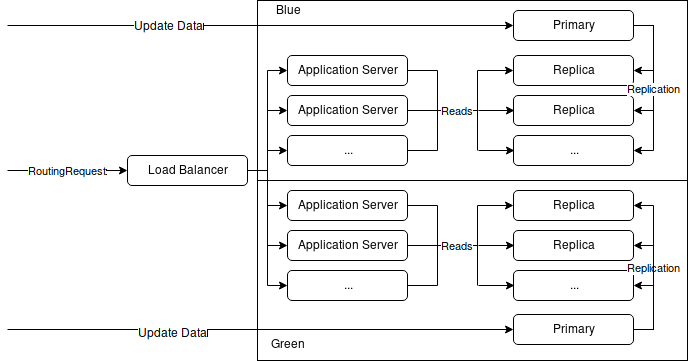
\includegraphics[width=.9\linewidth]{arch.png}
\caption{\label{fig:scaling}
Horizontal skalierbare Architektur der Anwendung}
\end{figure}

Jede der Zonen beinhaltet einen PostgreSQL Cluster. Ein PostgreSQL Cluster besteht aus mehreren Rechnern, die jeweils eine Instanz der Datenbank beherbergen. Einer dieser Rechner wird als \texttt{Primary} bezeichnet. Sämtliche Änderungen an den Daten erfolgen auf diesem Rechner. Die Änderungen werden anschließend auf die anderen Rechner übertragen. Die anderen Rechner werden als \texttt{Replica} bezeichnet. Auf sie kann nur lesend zugegriffen werden.

Die Replikation der Daten kann zum Beispiel über die Replikation des \ac{WAL} sichergestellt werden. Dieser Vorgang wird in im PostgreSQL Wiki beschrieben \cite{pgwiki}. Das \ac{WAL} beinhaltet alle Änderungen am Datenbestand. Bei einer Änderung wird die entsprechende Anweisung im \ac{WAL} protokolliert. Erst bei Ausführung des Commits einer Datenbanktransaktion werden die geänderten Daten als sichtbar angesehen. Jede Änderung besteht aus einem oder mehreren Einträgen im \ac{WAL}. Diese Einträge werden nicht geändert und es werden immer nur neue Einträge am Ende des Logs hinzugefügt.

Um den Datenbestand zu replizieren kann also das \ac{WAL} des \texttt{Primary} Rechners an die \texttt{Replica} Rechner übertragen werden. Da das Log nur erweitert und nie geändert wird, kann dies sehr effizient umgesetzt werden.

Dieser Aufbau ermöglicht die horizontale Skalierung des Systems. Bei Einsatz entsprechender Monitoring-Werkzeuge können während des Betriebs Flaschenhälse identifiziert werden. Je nachdem, ob der Flaschenhalts im Bereich der Application Server oder des PostgreSQL Clusters auftritt, können im entsprechenden Bereich mehr Rechner hinzugefügt werden. Durch die neuen Rechner kann der Flaschenhals beseitigt werden.

Die Aufteilung des Systems in die zwei Zonen hat den Vorteil, dass Änderungen am System immer in der gerade nicht aktiven Zone durchgeführt werden können. Bei Änderungen an den \ac{OSM} Daten oder dem Erhalt neuer historischer Preisdaten, kann so die Neuberechnung der Daten erfolgen ohne, dass das laufende System beeinträchtigt wird. Sobald die Berechnung fertig ist, kann der Load Balancer die aktuell aktive Zone wechseln und den Benutzern stehen aktuelle Daten zur Verfügung.

Mit dem hier beschriebenen System wäre es möglich das Anwendungszenario zu erfüllen und die Funktionalität der Anwendung vielen simultanen Benutzern zur Verfügung zu stellen. Die Aufgabenstellung lässt jedoch noch viele weitere sinnvolle Erweiterungen zu. Diese Erweiterungen werden im Folgenden beschrieben.

\section{Weitere Ansatzpunkte zur Erweiterung des Systems}
\label{sec:org85ddd52}

Dieser Abschnitt beschreibt weitere Ansatzpunkte, um das System zu erweitern und den Nutzen für die Benutzer dadurch zu erweitern. Die heutige Allgegenwärtigkeit von Smartphones erlaubt kontinuierliche Rückmeldungen an das System. Der Benutzer könnte sowohl den realen Verbrauch seines Fahrzeugs, als auch die tatsächlichen Benzinpreise an das System übermitteln.

Mit diesen Daten kann die Routenplanung und die Preisvorhersage verbessert werden. Diese Daten erlauben nicht nur eine Verbesserung der allgemeinen Vorhersagegüte, sondern erlauben auch eine individuelle Anpassung an den Benutzer. 

Die hier vorgestellte Architektur berücksichtigt dies nicht und wäre bei der Implementierung dieser Features erneut zu evaluieren.

\chapter{Ausblick}
Die vorgestellte Lösung hat seinen größten praktischen Nutzen sicherlich im Fernverkehr, insbesondere im Güterfernverkehr. Bei letzterem werden Lastkraftfahrzeuge eingesetzt, deren Tankkapazität mehrere hundert Liter umfasst. Durch die Benzinpreis-optimierte Routenplanung können hier erhebliche Kosten gespart werden. Ähnliches gilt für den Personenfernverkehr mit Bussen. Durch die eingesparten Spritkosten können Fahrkarten günstiger verkauft werden, was wiederum eventuell neue Kundschaft anlockt und somit in einer verstärkten Nutzung von Reisebussen resultiert. Dies hätte zusätzlich einen positiven ökologischen Nebeneffekt im Hinblick auf den Klimawandel. \\
\par
Die Planung des Bundesverkehrsministeriums zur Installation von 5000 Ladestationen für Elektroautos \cite{ladestations-planung} wirft die Überlegung in den Raum, ob Intellitank auch hierauf anwendbar ist. Mit dieser Investition soll auch ein einheitliches Bezahlsystem eingeführt werden. Laut einer Untersuchung der ISPEX AG \cite{oel-strom} folgt der Strompreis in seiner Entwicklung dem Ölpreis. Dies passt sehr gut in das Konzept von Intellitank. Probleme bereiten jedoch kostenlose Ladestationen für Supermarktkunden und die insgesamt noch limitierte Reichweite von Elektroautomobilen. Da der Besitzer sein Fahrzeug zu Hause aufladen kann, benötigt er für den Alltagsverkehr nicht zwingend ein Planungssystem für optimale Tankstrategien. Erst die flächendeckende Infrastruktur für Ladestationen macht Intellitank interessant für Besitzer von Elektrofahrzeugen, da sie somit auch über weite Strecken mit ihrem Fahrzeug reisen können. \\
\par 
Ein weiteres spannendes Einsatzgebiet für Intellitank bietet das Forschungsgebiet des Autonomous Driving. Ein selbstfahrendes Auto kann dann die Route Benzinpreis-optimal berechnen, so dass der Mitfahrer nur noch einsteigen muss und direkt losfahren kann. 

%-------------------------------------------------------------------------------
% APPENDIX
%-------------------------------------------------------------------------------
\newpage
\appendix

\chapter{Anleitungen}
\section*{Installationsanleitung}
\addcontentsline{toc}{section}{Installationsanleitung}
\label{label:installation}
Für die Installation wird von einem Linux System ausgegangen. Die Schritte sind für andere Betriebssysteme entsprechend anzupassen.

Zur Installation wird eine .zip-Datei namens 'RoutingService.zip' benötigt. Diese beinhaltet das Backend- und das Frontend-Setup, sowie eine fertig kompilierte Jar Datei.

Zusätzlich zu der .ZIP-Datei liegt anbei ein .sql-Dump.gz, welcher auf eine PostgreSql-Datenbank importiert werden muss. Die Anwendung wurde mit Postgresql 9.6.5 und PostGIS 2.3.3 getestet. Um die Datenbank aufzuspielen sind folgende Schritte notwendig.

\begin{lstlisting}
gunzip infocup.sql-dump.gz
psql infocup < infocup.sql-dump
\end{lstlisting}

Die Datenmenge ist recht groß. Deshalb sollte die Standardkonfiguration von Postgresql entsprechend angepasst werden.

Um die Jar Datei zu bauen wird das JDK8 und Maven benötigt. Während des Builds lädt Maven sowohl NodeJs als auch den Paket-Manager yarn herunter.

Um das Projekt zu generieren wird in den Ordner 'RoutingService' gewechselt und folgender Befehl ausgeführt:
\begin{lstlisting}
mvn clean install
\end{lstlisting}
Im Ordner {\em target} liegt nach erfolgreichem Build-Prozess die jar-Datei {\em RoutingService-1.0-SNAPSHOT.jar} vor.

\section*{Bedienungsanleitung}
\addcontentsline{toc}{section}{Bedienungsanleitung}

Um mit der Anwendung zu arbeiten, ohne selbst eine Datenbank aufzuspielen, kann die Demo Instanz genutzt werden. Diese ist unter \url{https://infocup.noshak.de} erreichbar. Der Benutzer \texttt{infocup} und das Passwort \texttt{predictp} werden für den Zugang benötigt.

Sofern die Installation aus vorherigem Abschnitt erfolgreich beendet wurde, kann man das Projekt mittels
\begin{lstlisting}
java -jar RoutingService-1.0-SNAPSHOT.jar \
  -D infocup.host="localhost:5432" \
  -D infocup.user="infocup"
\end{lstlisting}
starten.
Die übergebenen Properties \texttt{infocup.host} und \texttt{infocup.user} konfigurieren die Verbindung zur Datenbank und sind entsprechend anzupassen.

Wie in Abbildung \ref{fig:install1} zu sehen ist, gibt das Startup-Log die Adresse an, auf die der Server lauscht. In diesem Fall {\em 0.0.0.0:4567}, also abrufbar über {\em http://localhost:4567}.
\begin{figure}[H]
\centering
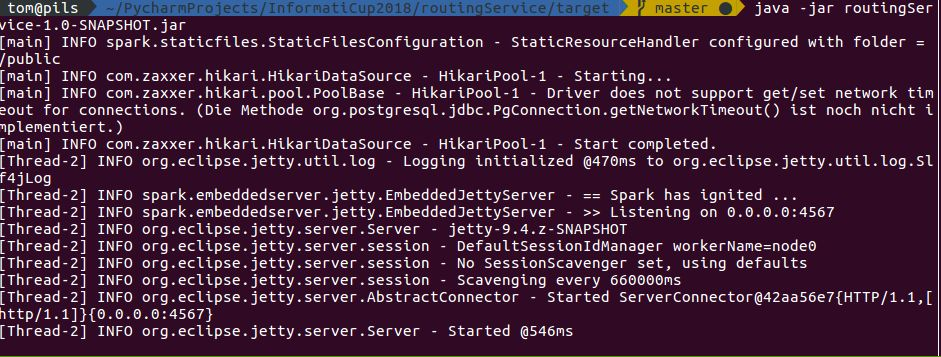
\includegraphics[width=1\linewidth]{install1.jpg}
\caption{Server-Log beim Starten des Projekts}
\label{fig:install1}
\end{figure}
Die Web-Anwendung bietet zwei wesentliche Funktionen.\\
Im unteren rechten Eck (siehe Abbildung \ref{fig:install2}) gibt es einen Button, der per Klick dem Benutzer die Möglichkeit eröffnet, entweder Preise vorherzusagen oder eine optimale Route berechnen zu lassen.
\begin{figure}[H]
\centering
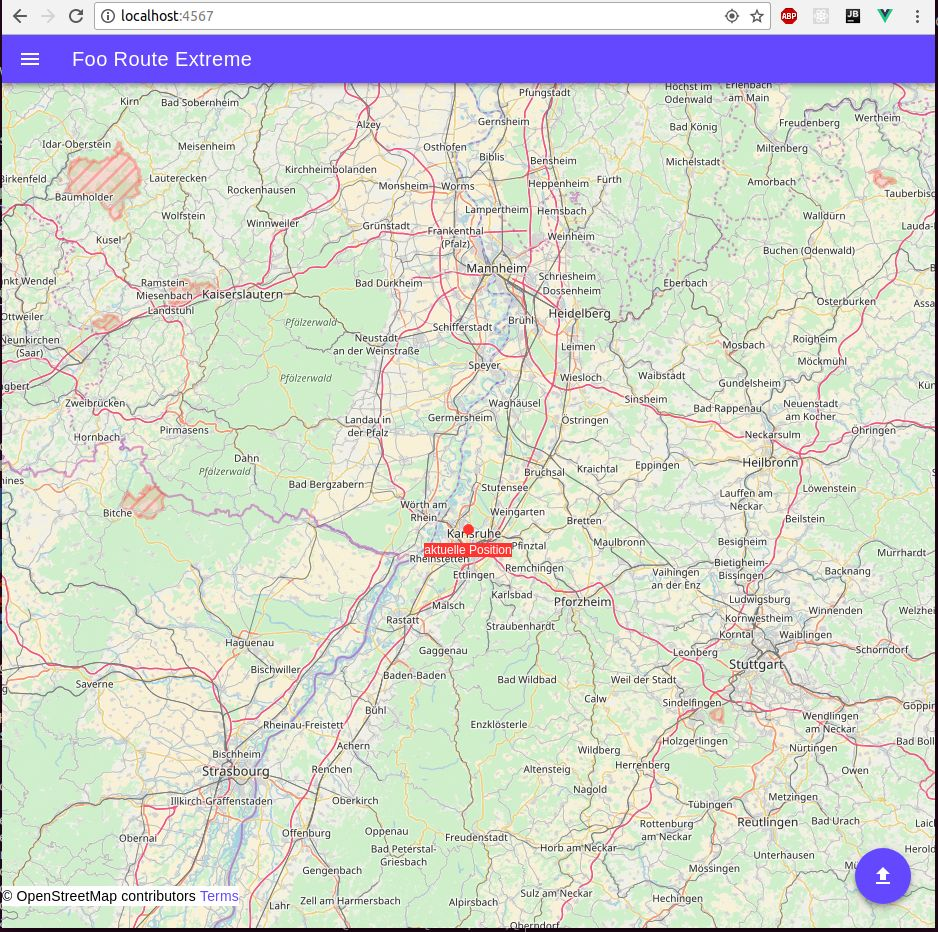
\includegraphics[width=0.6\linewidth]{install2.jpg}
\caption{grundlegende Oberfläche der Webanwendung}
\label{fig:install2}
\end{figure}
\clearpage

Die Buttons in Abbildung \ref{fig:install3} öffnen in beiden Fällen bei Klick einen File-Dialog zum Hochladen einer CSV-Datei.
Beim Klick auf den oberen Button besteht die Möglichkeit eine Tabelle, wie beispielsweise die Bertha-Benz-Memorial-Route, zu öffnen um eine optimale Tankstrategie zu berechnen. Beim Klick des unteren wird eine CSV-Datei erwartet, die Zeilen beinhaltet mit jeweils einer Tankstellen-ID und einem Datum, woraufhin eine Preisvorhersage berechnet wird.
\begin{figure}[H]
\centering
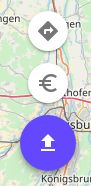
\includegraphics[width=50px]{install3.jpg}
\caption{die Benutzer-Interaktionsmöglichkeiten}
\label{fig:install3}
\end{figure}

\subsection{Routen-Berechnung}
Nach Eingabe der Bertha-Benz-Memorial-Route ist diese auf der Karte zu sehen (siehe Abbildung \ref{fig:install4}). Die Geo-Punkte der jeweiligen Tankstellen werden aus der Datenbank entnommen und auf die Karte projiziert. Ein blauer Punkt entspricht einer Tankstelle (Stopp), der grüne Punkt entspricht dem Startpunkt der Route, der beschriftete, rote Punkt der aktuellen Position und der zweite rote Punkt der letzten Station auf der Route.
\begin{figure}[H]
\centering
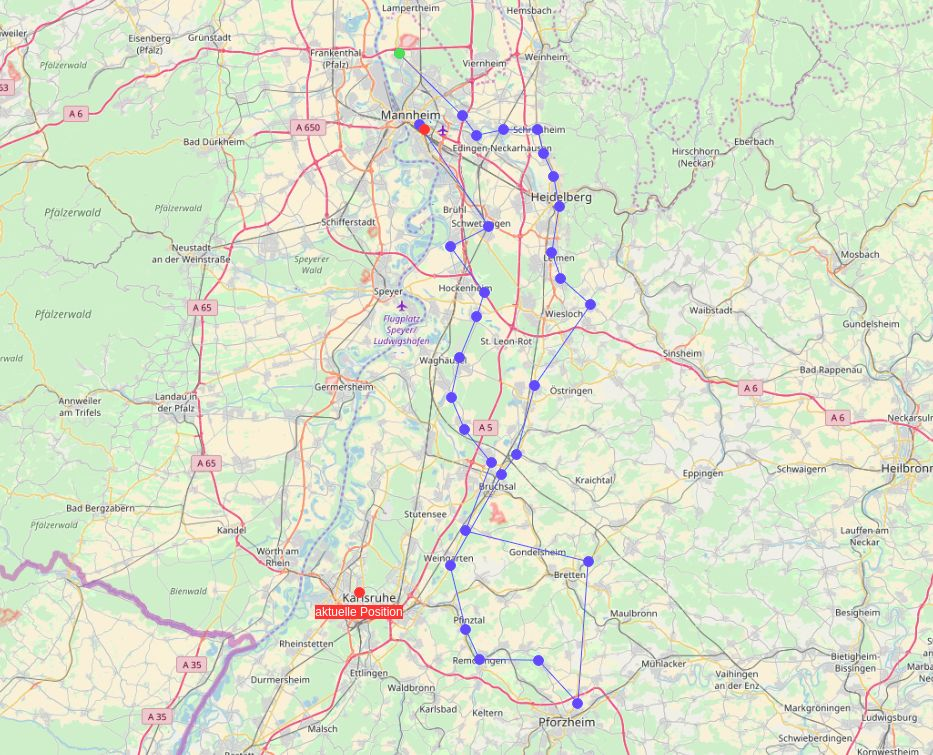
\includegraphics[width=0.6\linewidth]{install4.jpg}
\caption{Anzeige einer Tankroute}
\label{fig:install4}
\end{figure}
Neben der Karte kann ein Reiter eingeblendet werden, indem man den Navigations-Button oben links drückt (siehe Abbildung \ref{fig:install5}). Dieser dient dazu, die errechneten Tankfüllungen pro Routen-Stopp anzuzeigen.
\begin{figure}[H]
\centering
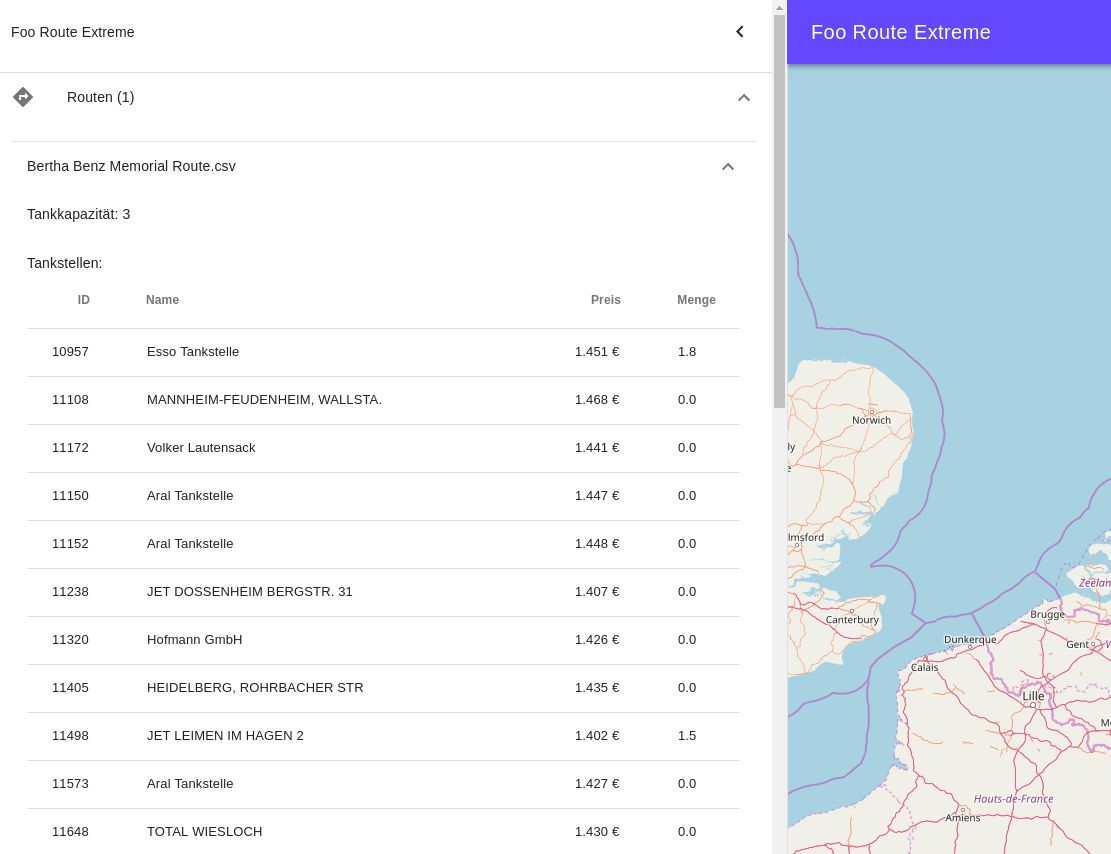
\includegraphics[width=0.8\linewidth]{install5.jpg}
\caption{die errechneten Tankfüllungen für die Route}
\label{fig:install5}
\end{figure}

\subsection{Preisvorhersage}

Wie auch bei der Routen-Berechnung werden bei der Funktion 'Preisvorhersage' alle Tankstellen in Form eines blauen Punktes auf der Karte illustriert (siehe Abbildung \ref{fig:install6}).
Der Unterschied ist jedoch, dass die jeweiligen Tankstellen nicht untereinander (wie bei einer Route) verbunden sind.
\begin{figure}[H]
\centering
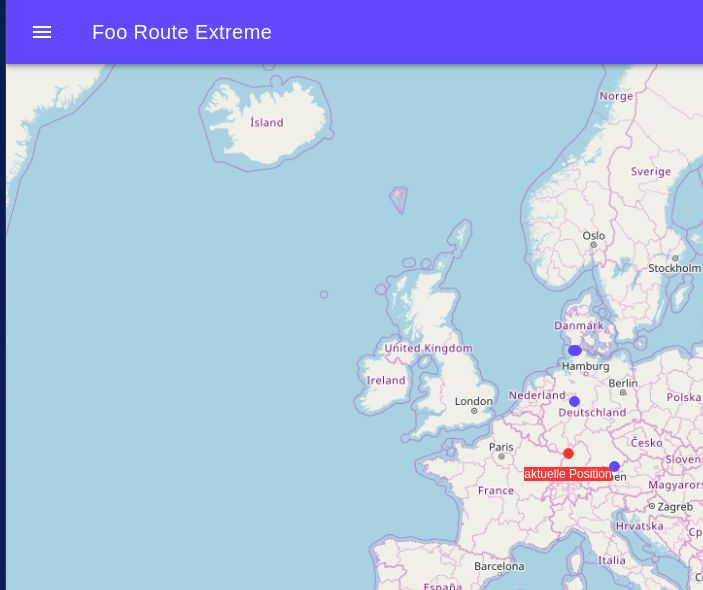
\includegraphics[width=0.6\linewidth]{install6.jpg}
\caption{die Tankstellen auf der Karte bei einer Preisvorhersage}
\label{fig:install6}
\end{figure}
Durch Klick auf die Top-Navigation, um den Reiter zu öffnen, werden die vorhergesagten Preise pro Tankstelle angezeigt (siehe Abb. \ref{fig:install7}).
\begin{figure}[H]
\centering
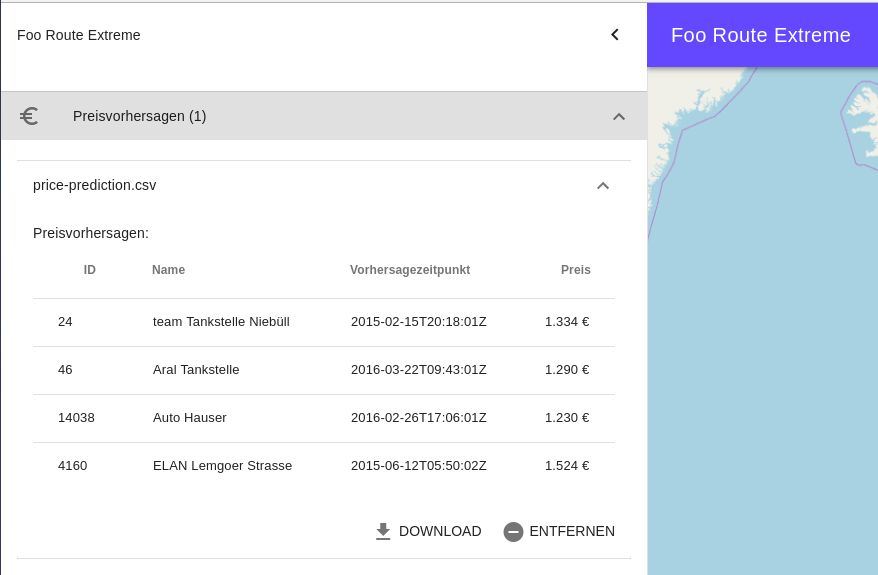
\includegraphics[width=0.8\linewidth]{install7.jpg}
\caption{die errechneten Preise zu den jeweiligen Daten}
\label{fig:install7}
\end{figure}

Zusätzlich bietet der Reiter die Möglichkeit die Routen zu löschen oder herunterzuladen.

%%%%%%%%%%%%%%%%%%%%%%%%%%%%%%%%%%%%%%%5
% BIBLATEX
% Benutzt man das "biblatex"-Paket, muß man folgendes schreiben:
\def\refname{Literaturverzeichnis}
\printbibliography[sorting=none]
%%%%%%%%%%%%%%%%%%%%%%%%%%%%%%%%%%%%%%%5

\end{document}

%-------------------------------------------------------------------------------
% SNIPPETS
%-------------------------------------------------------------------------------

%\begin{figure}[!ht]
%	\centering
%	\includegraphics[width=0.8\textwidth]{file_name}
%	\caption{}
%	\centering
%	\label{label:file_name}
%\end{figure}

%\begin{figure}[!ht]
%	\centering
%	\includegraphics[width=0.8\textwidth]{graph}
%	\caption{Blood pressure ranges and associated level of hypertension (American Heart Association, 2013).}
%	\centering
%	\label{label:graph}
%\end{figure}

%\begin{wrapfigure}{r}{0.30\textwidth}
%	\vspace{-40pt}
%	\begin{center}
%		\includegraphics[width=0.29\textwidth]{file_name}
%	\end{center}
%	\vspace{-20pt}
%	\caption{}
%	\label{label:file_name}
%\end{wrapfigure}

%\begin{wrapfigure}{r}{0.45\textwidth}
%	\begin{center}
%		\includegraphics[width=0.29\textwidth]{manometer}
%	\end{center}
%	\caption{Aneroid sphygmomanometer with stethoscope (Medicalexpo, 2012).}
%	\label{label:manometer}
%\end{wrapfigure}

%\begin{table}[!ht]\footnotesize
%	\centering
%	\begin{tabular}{cccccc}
%	\toprule
%	\multicolumn{2}{c} {Pearson's correlation test} & \multicolumn{4}{c} {Independent t-test} \\
%	\midrule	
%	\multicolumn{2}{c} {Gender} & \multicolumn{2}{c} {Activity level} & \multicolumn{2}{c} {Gender} \\
%	\midrule
%	Males & Females & 1st level & 6th level & Males & Females \\
%	\midrule
%	\multicolumn{2}{c} {BMI vs. SP} & \multicolumn{2}{c} {Systolic pressure} & \multicolumn{2}{c} {Systolic Pressure} \\
%	\multicolumn{2}{c} {BMI vs. DP} & \multicolumn{2}{c} {Diastolic pressure} & \multicolumn{2}{c} {Diastolic pressure} \\
%	\multicolumn{2}{c} {BMI vs. MAP} & \multicolumn{2}{c} {MAP} & \multicolumn{2}{c} {MAP} \\
%	\multicolumn{2}{c} {W:H ratio vs. SP} & \multicolumn{2}{c} {BMI} & \multicolumn{2}{c} {BMI} \\
%	\multicolumn{2}{c} {W:H ratio vs. DP} & \multicolumn{2}{c} {W:H ratio} & \multicolumn{2}{c} {W:H ratio} \\
%	\multicolumn{2}{c} {W:H ratio vs. MAP} & \multicolumn{2}{c} {\% Body fat} & \multicolumn{2}{c} {\% Body fat} \\
%	\multicolumn{2}{c} {} & \multicolumn{2}{c} {Height} & \multicolumn{2}{c} {Height} \\
%	\multicolumn{2}{c} {} & \multicolumn{2}{c} {Weight} & \multicolumn{2}{c} {Weight} \\
%	\multicolumn{2}{c} {} & \multicolumn{2}{c} {Heart rate} & \multicolumn{2}{c} {Heart rate} \\
%	\bottomrule
%	\end{tabular}
%	\caption{Parameters that were analysed and related statistical test performed for current study. BMI - body mass index; SP - systolic pressure; DP - diastolic pressure; MAP - mean arterial pressure; W:H ratio - waist to hip ratio.}
%	\label{label:tests}
%\end{table}
